\documentclass[11pt,oneside]{article}

\usepackage[T1]{fontenc}
\usepackage[utf8]{inputenc}
\usepackage{newtxtext}
\usepackage{amsmath,amssymb,amsthm,mathtools}
\usepackage{newtxmath}
\usepackage[letterpaper,margin=1in,headheight=15pt]{geometry}
\usepackage{microtype}
\usepackage{bm}
\usepackage{booktabs,longtable,array,tabularx,multirow}
\usepackage{enumitem}
\usepackage{graphicx}
\usepackage{tikz}
\usepackage{pgfplots}
\pgfplotsset{compat=1.18}
\usepackage[most]{tcolorbox}
\usepackage[dvipsnames]{xcolor}
\usepackage{fancyhdr}
\usepackage{titlesec}
\usepackage{hyperref}
\usepackage{bookmark}
\usepackage[nameinlink,noabbrev]{cleveref}
\usepackage{upquote}

\definecolor{FabiusBlue}{HTML}{1F4E79}
\definecolor{FabiusTeal}{HTML}{2A6F74}
\definecolor{FabiusGold}{HTML}{A66B13}
\definecolor{FabiusGray}{HTML}{4B5563}
\definecolor{FabiusPale}{HTML}{F3F7FA}
\definecolor{FabiusWarn}{HTML}{FFF6E5}

\hypersetup{
  colorlinks=true,
  linkcolor=FabiusBlue,
  citecolor=FabiusTeal,
  urlcolor=FabiusGold,
  pdftitle={The Fabius Function and Rvachev's Up Function},
  pdfauthor={Exposition based on Vladimir Reshetnikov's Lean development},
  pdfsubject={Fabius function, Rvachev up-function, dyadic values, asymptotics},
  pdfkeywords={Fabius function, Rvachev up, dyadic rational, Thue-Morse, Lambert W, saddle point}
}

\pagestyle{fancy}
\fancyhf{}
\fancyhead[L]{\small The Fabius Function and Rvachev's Up Function}
\fancyhead[R]{\small\nouppercase{\leftmark}}
\fancyfoot[C]{\thepage}
\renewcommand{\headrulewidth}{0.4pt}

\titleformat{\section}{\Large\bfseries\color{FabiusBlue}}{\thesection}{0.65em}{}
\titleformat{\subsection}{\large\bfseries\color{FabiusTeal}}{\thesubsection}{0.65em}{}
\titleformat{\subsubsection}{\normalsize\bfseries\color{FabiusGray}}{\thesubsubsection}{0.65em}{}

\setlist[itemize]{leftmargin=1.55em,itemsep=0.3em,topsep=0.5em}
\setlist[enumerate]{leftmargin=1.8em,itemsep=0.35em,topsep=0.5em}
\setlength{\parindent}{1.25em}
\setlength{\parskip}{0.15em}
\allowdisplaybreaks
\emergencystretch=2em

\newtheorem{theorem}{Theorem}[section]
\newtheorem{proposition}[theorem]{Proposition}
\newtheorem{lemma}[theorem]{Lemma}
\newtheorem{corollary}[theorem]{Corollary}
\newtheorem{conjecture}[theorem]{Conjecture}
\theoremstyle{definition}
\newtheorem{definition}[theorem]{Definition}
\newtheorem{example}[theorem]{Example}
\newtheorem{algorithm}[theorem]{Algorithm}
\theoremstyle{remark}
\newtheorem{remark}[theorem]{Remark}

\newtcolorbox{keybox}[1][]{
  enhanced,breakable,colback=FabiusPale,colframe=FabiusBlue,
  boxrule=0.6pt,arc=1.2mm,left=1.5mm,right=1.5mm,top=1.2mm,bottom=1.2mm,
  title={#1},fonttitle=\bfseries
}
\newtcolorbox{warningbox}[1][]{
  enhanced,breakable,colback=FabiusWarn,colframe=FabiusGold,
  boxrule=0.6pt,arc=1.2mm,left=1.5mm,right=1.5mm,top=1.2mm,bottom=1.2mm,
  title={#1},fonttitle=\bfseries
}

\newcommand{\upf}{\operatorname{up}}
\newcommand{\sinc}{\operatorname{sinc}}
\newcommand{\den}{\operatorname{den}}
\newcommand{\ord}{\operatorname{ord}}
\newcommand{\supp}{\operatorname{supp}}
\newcommand{\wt}{w_2}
\newcommand{\epsTM}{\varepsilon}
\newcommand{\dd}{\,\mathrm d}
\newcommand{\ii}{\mathrm i}
\newcommand{\ee}{\mathrm e}
\newcommand{\E}{\mathbb E}
\newcommand{\Pp}{\mathbb P}
\newcommand{\N}{\mathbb N}
\newcommand{\Z}{\mathbb Z}
\newcommand{\Q}{\mathbb Q}
\newcommand{\R}{\mathbb R}
\newcommand{\C}{\mathbb C}
\newcommand{\Thetaf}{\Theta}
\newcommand{\Lam}{\lambda}
\newcommand{\Ltwo}{L}
\newcommand{\PsiPer}{\Psi}
\newcommand{\Fourier}{\widehat{\upf}}
\newcommand{\gaussbinom}[3]{\genfrac{[}{]}{0pt}{}{#1}{#2}_{#3}}
\newcommand{\abs}[1]{\left\lvert#1\right\rvert}
\newcommand{\norm}[1]{\left\lVert#1\right\rVert}
\newcommand{\set}[1]{\left\{#1\right\}}
\newcommand{\floor}[1]{\left\lfloor#1\right\rfloor}
\newcommand{\ceil}[1]{\left\lceil#1\right\rceil}
\newcommand{\brak}[1]{\left(#1\right)}

\crefname{algorithm}{algorithm}{algorithms}
\Crefname{algorithm}{Algorithm}{Algorithms}

\begin{document}

\hypersetup{pageanchor=false}
\begin{titlepage}
\centering
\vspace*{1.0in}
{\Huge\bfseries\color{FabiusBlue} The Fabius Function\\[0.18in]
and Rvachev's Up Function\par}
\vspace{0.35in}
{\Large Smoothness, exact dyadic arithmetic, Fourier structure,\\
and sharp endpoint asymptotics\par}
\vspace{0.7in}
{\large A human-readable exposition based on the complete Lean development\\
in \texttt{VladimirReshetnikov/ProveIt}\par}
\vfill
\begin{minipage}{0.84\textwidth}
\small
This article synthesizes the formal development in
\href{https://github.com/VladimirReshetnikov/ProveIt/tree/main/Analysis/FabiusFunction}
{\texttt{Analysis/FabiusFunction}} on the repository's main branch as inspected in
August 2026.  It distinguishes the bounded cumulative-distribution version of the
Fabius function from its signed global extension, and it states conjectural material
as conjectural.  The proofs below are ordinary mathematical proofs; the Lean source
provides a machine-checked refinement of the same dependency structure.
\end{minipage}
\vfill
{\large August 2026\par}
\end{titlepage}
\hypersetup{pageanchor=true}

\begin{abstract}
The Fabius function is a canonical smooth transition from $0$ to $1$ whose
self-similarity is governed by the differential equation $F'(x)=2F(2x)$.
Its even twin, Rvachev's compactly supported function $\upf$, is the unique
normalized smooth solution of
\[
  \upf'(x)=2\bigl(\upf(2x+1)-\upf(2x-1)\bigr),
  \qquad \supp \upf=[-1,1],\qquad \upf(0)=1.
\]
These functions simultaneously belong to probability, harmonic analysis,
combinatorics, exact arithmetic, approximation theory, and asymptotic analysis.
The present article develops their equivalent constructions, existence and
uniqueness, smoothness and failure of analyticity on the support, Fourier products,
Poisson summation, moments, polynomial and Legendre expansions, and the signed
global extension controlled by the Thue--Morse sequence.

Particular attention is paid to two topics.  First, every dyadic value is rational.
We prove both a closed finite Thue--Morse formula and a recursive Taylor-block
formula that removes the highest binary digit of the numerator.  These formulas
lead to exact algorithms, denominator bounds, $2$-adic valuations, the integral and
odd Reshetnikov numbers, and finite $q$-binomial identities.  Second, we derive the
sharp small-$x$ expansion of $\log F(x)$.  Its natural coordinate is the lower
Lambert phase
\[
  \Lam(x)=-\frac{W_{-1}(-x\log 2)}{\log 2},
  \qquad \Lam(x)2^{-\Lam(x)}=x,
\]
not merely $-\log_2x$.  The expansion contains an explicit, nonconstant, smooth
one-periodic term sampled at $\Lam(x)$; omitting this term makes the often quoted
$O(1/\log x)$ remainder false.  We give the exact periodic Laplace decomposition,
its Gamma--zeta Fourier coefficients and mean, the corrected Lambert form, an
elementary logarithmic form, the first periodic saddle correction, and the
full all-orders expansion in inverse powers of $\Lam(x)$.
\end{abstract}

\tableofcontents
\clearpage

\section{Orientation: three functions, not one}

The notation surrounding the Fabius function is historically inconsistent.
One source writes a globally defined signed function as $F$; another reserves $F$
for the increasing function on $[0,1]$; still another begins with the compact bump
$\upf$.  Mixing these conventions is harmless for some identities and disastrous
for others.  We therefore fix the following three objects from the outset.

\begin{definition}[The bounded Fabius function]\label{def:bounded-F}
The bounded Fabius function is the unique map $F\colon\R\to[0,1]$ satisfying
\begin{align}
  F(x)&=0 &&(x\le 0),\label{eq:F-left}\\
  F(x)&=1 &&(x\ge 1),\label{eq:F-right}\\
  F(1-x)&=1-F(x) &&(0\le x\le1),\label{eq:F-sym}\\
  F'(x)&=2F(2x) &&(0\le x\le\tfrac12),\label{eq:F-diff-local}
\end{align}
and $F\in C^\infty(\R)$.  We use the clamped extension in
\eqref{eq:F-left}--\eqref{eq:F-right}, even when only the restriction to $[0,1]$
is under discussion.
\end{definition}

\begin{definition}[Rvachev's up-function]\label{def:up-from-F}
The up-function associated with $F$ is
\begin{equation}\label{eq:up-from-F}
  \upf(x)=
  \begin{cases}
    F(x+1),&x\le0,\\
    F(1-x),&x>0.
  \end{cases}
\end{equation}
Thus $\upf$ is supported in $[-1,1]$, and on that interval
\begin{equation}\label{eq:F-up-bridge}
  F(x)=\upf(x-1)\quad(0\le x\le1),
  \qquad
  \upf(x)=1-F(x)\quad(0\le x\le1).
\end{equation}
\end{definition}

Let $\wt(n)$ denote the number of $1$'s in the binary expansion of $n$, and put
\begin{equation}\label{eq:TM-sign}
  \epsTM_n=(-1)^{\wt(n)}.
\end{equation}
The elementary identities
\begin{equation}\label{eq:TM-scaling}
  \epsTM_{2n}=\epsTM_n,
  \qquad
  \epsTM_{2n+1}=-\epsTM_n
\end{equation}
are the algebraic engine behind the global self-similarity.

\begin{definition}[The signed global extension]\label{def:global-theta}
Define
\begin{equation}\label{eq:global-theta}
  \Thetaf(x)=\sum_{n=0}^{\infty}\epsTM_n\,
  \upf(x-2n-1).
\end{equation}
The sum is locally finite, because the supports of the summands have disjoint
interiors.  On the band $[2m,2m+2]$,
\begin{equation}\label{eq:theta-band}
  \Thetaf(x)=\epsTM_m\,\upf(x-2m-1).
\end{equation}
In particular, $\Thetaf=F$ on $[0,1]$ and $\Thetaf(x)=0$ for $x\le0$.
Unlike the bounded $F$, however, $\Thetaf$ is signed and nonconstant beyond $1$.
\end{definition}

We will usually write $F$ for the bounded function and $\Thetaf$ for the signed
extension.  Statements from older literature that use $F$ globally are to be read
with $F$ replaced by $\Thetaf$.

\subsection{Historical coordinates}

The same distribution or function appeared independently in several guises: in
work of Jessen and Wintner on infinite convolutions, in Fabius's probabilistic
example of a nowhere analytic $C^\infty$ function, in Rvachev's compactly supported
solutions of functional-differential equations, and later in work of Kirov--Totkov,
Arias de Reyna, Schnabl, and others.  Arias de Reyna's 1982 paper gives a systematic
construction and a large collection of identities; his later paper develops the
arithmetic of the dyadic values.  The modern formal development on which this
article is based proves the results of both papers, supplies missing analytic
bridges, corrects several endpoint and normalization defects, and extends the
asymptotic theory substantially.

The most useful conceptual slogan is this:

\begin{keybox}[One object, four viewpoints]
The bounded $F$ is a cumulative distribution function; $\upf$ is the density of a
centered version of the same random series; $\widehat{\upf}$ is an infinite sinc
product; and $\Thetaf$ is the Thue--Morse signed global continuation satisfying a
pure dilation differential equation.
\end{keybox}

\section{Probability and infinite convolution}

\subsection{The random series}

Let $(U_n)_{n\ge1}$ be independent random variables, each uniformly distributed on
$[0,1]$, and set
\begin{equation}\label{eq:X-random-series}
  X=\sum_{n=1}^{\infty}\frac{U_n}{2^n}.
\end{equation}
The series converges almost surely and in every $L^p$, and $0\le X\le1$.  Its law is
symmetric about $1/2$, since replacing each $U_n$ by $1-U_n$ changes $X$ into
$1-X$ without changing the joint law.

It is often cleaner to center and rescale:
\begin{equation}\label{eq:Y-random-series}
  Y=2X-1=\sum_{j=0}^{\infty}V_j,
  \qquad
  V_j\sim\operatorname{Unif}\bigl[-2^{-j-1},2^{-j-1}\bigr],
\end{equation}
with the $V_j$ independent.  The support widths sum to $1$, so $Y\in[-1,1]$.

\begin{theorem}[Probabilistic realization]\label{thm:prob-realization}
The random variable $X$ has cumulative distribution function $F$, and $Y=2X-1$
has density $\upf$.  Equivalently,
\begin{equation}\label{eq:F-as-probability}
  F(x)=\Pp(X\le x),\qquad 0\le x\le1,
\end{equation}
and
\begin{equation}\label{eq:up-density}
  \Pp(Y\in A)=\int_A\upf(t)\dd t
\end{equation}
for every Borel set $A\subseteq\R$.
\end{theorem}

\begin{proof}
For a finite truncation $Y_N=\sum_{j=0}^N V_j$, the law is the convolution of the
uniform measures on the indicated intervals.  Its characteristic function, in the
Fourier convention $\widehat g(z)=\int g(t)e^{-2\pi\ii tz}\dd t$, is
\begin{equation}\label{eq:finite-characteristic}
  \prod_{j=0}^{N}\frac{\sin(\pi z/2^j)}{\pi z/2^j}.
\end{equation}
The random variables $Y_N$ converge almost surely to $Y$, so their laws converge
weakly.  In \cref{sec:fourier} we prove that the limiting product is the Fourier
transform of a $C^\infty$ density supported in $[-1,1]$; call that density $u$.
Consequently $Y$ has density $u$.

Let $H$ be the distribution function of $X=(Y+1)/2$.  On $-1\le y\le0$,
\[
  u(y)=\frac12 H'\!\left(\frac{y+1}{2}\right).
\]
The refinement identity proved below implies
$\frac12H'((y+1)/2)=H(y+1)$.  Hence $u(y)=H(y+1)$ on the left half of the support.
Symmetry gives $u(y)=H(1-y)$ on the right half.  Thus $H$ and $u$ satisfy exactly
the bridge in \eqref{eq:up-from-F}.  The uniqueness theorem in
\cref{sec:existence-uniqueness} identifies $H=F$ and $u=\upf$.
\end{proof}

The theorem also gives the left-half identity that appeared in the original
probabilistic construction:
\begin{equation}\label{eq:up-left-prob}
  \upf(x)=\Pp\left(\sum_{n=1}^{\infty}\frac{U_n}{2^n}\le x+1\right),
  \qquad -1\le x\le0.
\end{equation}
The apparent mismatch between ``$F$ is a CDF'' and ``$\upf$ is a density'' is not a
contradiction: the differential self-similarity turns the left half of the density
of $Y$ into the CDF of $X$.

\subsection{The refinement and delay-differential equations}

Separate the first summand in \eqref{eq:Y-random-series}:
\begin{equation}\label{eq:Y-decompose}
  Y=V_0+\frac12Y',
\end{equation}
where $V_0\sim\operatorname{Unif}[-1/2,1/2]$ and $Y'$ is an independent copy of
$Y$.  The density of $Y'/2$ is $2\upf(2x)$.  Convolution with the density
$\mathbf1_{[-1/2,1/2]}$ gives the integral refinement law
\begin{equation}\label{eq:up-integral-refinement}
  \upf(x)=\int_{-1/2}^{1/2}2\upf\bigl(2(x-v)\bigr)\dd v
         =\int_{2x-1}^{2x+1}\upf(t)\dd t.
\end{equation}
Differentiating yields Rvachev's equation.

\begin{theorem}[Rvachev equation]\label{thm:rvachev-equation}
For every $x\in\R$,
\begin{equation}\label{eq:rvachev-equation}
  \upf'(x)=2\bigl(\upf(2x+1)-\upf(2x-1)\bigr).
\end{equation}
Moreover $\upf$ is even, nonnegative, supported in $[-1,1]$, normalized by
\begin{equation}\label{eq:up-normalization}
  \upf(0)=1,
  \qquad
  \int_{\R}\upf(x)\dd x=1.
\end{equation}
\end{theorem}

\begin{proof}
Equation \eqref{eq:rvachev-equation} follows from the fundamental theorem of
calculus applied to \eqref{eq:up-integral-refinement}.  The distribution of $Y$ is
symmetric, hence $\upf$ is even.  Its nonzero set is contained in $[-1,1]$
because the sum of the half-widths in \eqref{eq:Y-random-series} is $1$.  Its
closed (topological) support is exactly $[-1,1]$: every open subinterval of
$(-1,1)$ receives positive mass from a suitable finite convolution, while the
remaining tail can be confined to an arbitrarily small interval with positive
probability.  Normalization of the integral is the
normalization of a probability density.

Finally, put $x=0$ in \eqref{eq:up-integral-refinement}.  The integral is the total
mass on $[-1,1]$, so $\upf(0)=1$.
\end{proof}

\begin{corollary}[The local Fabius equation]\label{cor:F-differential}
The function $F(x)=\upf(x-1)$ on $[0,1]$ satisfies
\begin{equation}\label{eq:F-local-again}
  F'(x)=2F(2x),\qquad 0\le x\le\tfrac12.
\end{equation}
It also satisfies $F(1-x)=1-F(x)$.
\end{corollary}

\begin{proof}
For $0\le x\le1/2$, use \eqref{eq:rvachev-equation} at $x-1$:
\[
 F'(x)=\upf'(x-1)
 =2\bigl(\upf(2x-1)-\upf(2x-3)\bigr)=2\upf(2x-1)=2F(2x),
\]
because $2x-3\le-2$ lies outside the support.  Symmetry of $X$ about $1/2$ and
continuity of its law imply
$F(1-x)=\Pp(X\le1-x)=\Pp(X\ge x)=1-F(x)$.
\end{proof}

\subsection{Finite convolutions and constructive approximants}

Let
\begin{equation}\label{eq:rho-j}
  \rho_j(x)=2^j\mathbf1_{[-2^{-j-1},2^{-j-1}]}(x),
  \qquad
  u_N=\rho_0*\rho_1*\cdots*\rho_N.
\end{equation}
Then $u_N$ is a compactly supported piecewise polynomial density, and
\begin{equation}\label{eq:uN-Fourier}
  \widehat{u_N}(z)=\prod_{j=0}^{N}\sinc\left(\frac{\pi z}{2^j}\right),
  \qquad \sinc z=\begin{cases}\sin z/z,&z\ne0,\\1,&z=0.\end{cases}
\end{equation}
For every fixed $m$, the products converge in the weighted $L^1$ norm
$\int(1+|z|)^m|\cdot|\dd z$.  Fourier inversion therefore gives
\begin{equation}\label{eq:uN-Cm}
  u_N\longrightarrow\upf\quad\text{in }C^m(\R)
\end{equation}
for every $m$.  This is an explicit constructive existence proof, and it also
explains why increasingly many convolutions produce an increasingly flat bump.

A related discrete approximation starts with the polynomials
\begin{equation}\label{eq:partition-polynomials}
  p_0(x)=1,
  \qquad
  p_{m+1}(x)=p_m(x)\bigl(1+x+\cdots+x^{2^{m+1}-1}\bigr).
\end{equation}
The coefficient of $x^j$ in
$\prod_{r=1}^m(1+x+\cdots+x^{2^r-1})$ counts restricted digit sums and supplies
the height of a dyadic step approximant.  With half-weights at cell endpoints,
these step functions converge pointwise to $\upf$; without the half-weights the
endpoint statement is false.  The weak convergence is simply the convergence of
the finite random sums, while continuity of the limiting density upgrades it to
the stated pointwise limit.

\section{Existence, uniqueness, monotonicity, and support}\label{sec:existence-uniqueness}

\subsection{Rapid decay of the sinc product}

For $z\in\C$ define
\begin{equation}\label{eq:Phi-product}
  \Phi(z)=\prod_{j=0}^{\infty}\sinc\left(\frac{\pi z}{2^j}\right).
\end{equation}
Since $1-\sinc w=O(w^2)$ as $w\to0$, the product converges uniformly on compact
subsets of $\C$ and defines an entire even function.  On the real axis it decays
faster than every power.

\begin{lemma}[Schwartz decay]\label{lem:Phi-Schwartz}
For each integer $N\ge0$ there is a constant $C_N$ such that
\begin{equation}\label{eq:Phi-Schwartz-bound}
  |\Phi(t)|\le C_N(1+|t|)^{-N},\qquad t\in\R.
\end{equation}
The same is true after any fixed number of derivatives.
\end{lemma}

\begin{proof}
For real $y$,
\[
  |\sinc y|\le\min\{1,|y|^{-1}\}.
\]
Fix $N$ and retain the first $N$ factors of \eqref{eq:Phi-product}.  Their product
is $O(|t|^{-N})$, while every remaining factor has absolute value at most $1$.
This proves \eqref{eq:Phi-Schwartz-bound} away from a bounded interval; continuity
handles the interval.  Derivatives are finite sums of products in which finitely
many factors are differentiated.  The differentiated sinc factors have the same
type of polynomial bound, and one may retain additional undifferentiated factors
to obtain arbitrarily high decay.
\end{proof}

Consequently the inverse Fourier integral
\begin{equation}\label{eq:up-inverse-def}
  u(x)=\int_{\R}\Phi(t)e^{2\pi\ii tx}\dd t
\end{equation}
converges absolutely with all derivatives.  It gives a Schwartz function.  On the
other hand, $\Phi$ is the characteristic function of the random series $Y$, whose
law is supported in $[-1,1]$.  Hence $u$ is the density of that law and vanishes
outside $[-1,1]$.  This proves existence of a smooth compactly supported solution.

\subsection{Fourier uniqueness}

The Fourier transform turns the delay-differential equation into a one-step
refinement equation.

\begin{lemma}[Transform of Rvachev's equation]\label{lem:transform-delay}
Let $u\in C^1(\R)$ have compact support and satisfy
\[
  u'(x)=k\bigl(u(2x+1)-u(2x-1)\bigr).
\]
Then
\begin{equation}\label{eq:transform-delay-k}
  \widehat u(z)=\frac{k}{2}\sinc(\pi z)\,\widehat u(z/2).
\end{equation}
If $\widehat u(0)\ne0$, necessarily $k=2$.
\end{lemma}

\begin{proof}
Integration by parts gives
$\widehat{u'}(z)=2\pi\ii z\widehat u(z)$.  In the first shifted term put
$y=2x+1$, and in the second put $y=2x-1$.  The right-hand side transforms to
\[
  \frac{k}{2}\bigl(e^{\pi\ii z}-e^{-\pi\ii z}\bigr)\widehat u(z/2)
  =k\ii\sin(\pi z)\widehat u(z/2).
\]
Division by $2\pi\ii z$, with the value at $z=0$ filled in continuously, proves
\eqref{eq:transform-delay-k}.  Letting $z\to0$ gives
$\widehat u(0)=(k/2)\widehat u(0)$, hence $k=2$ when the integral of $u$ is nonzero.
\end{proof}

For $k=2$, iteration gives
\begin{equation}\label{eq:transform-iterate}
  \widehat u(z)=\left(\prod_{j=0}^{N-1}
  \sinc\left(\frac{\pi z}{2^j}\right)\right)\widehat u(z/2^N).
\end{equation}
As $N\to\infty$, continuity at the origin yields
\begin{equation}\label{eq:up-Fourier-product}
  \widehat u(z)=\widehat u(0)\Phi(z).
\end{equation}

\begin{theorem}[Existence and uniqueness]\label{thm:existence-uniqueness}
There is a unique $C^\infty$ function $u\colon\R\to\R$ with compact support,
$u(0)=1$, and
\begin{equation}\label{eq:unique-up-equation}
  u'(x)=2\bigl(u(2x+1)-u(2x-1)\bigr).
\end{equation}
It is $\upf$.  Equivalently, there is a unique bounded Fabius function in the
sense of \cref{def:bounded-F}.
\end{theorem}

\begin{proof}
Existence was obtained from the inverse transform \eqref{eq:up-inverse-def}.  Its
integral is $\Phi(0)=1$, and the refinement equation follows either by Fourier
inversion or by conditioning as in \cref{thm:rvachev-equation}.  The value at zero
is $1$ by \eqref{eq:up-integral-refinement}.

For uniqueness, let $u$ be any other solution and write $U=\widehat u$.
Compact support makes $U$ entire, and the differential equation gives
$U(z)=\sinc(\pi z)U(z/2)$.  We first show that $U(0)\ne0$.  Otherwise, if $U$ were
not identically zero, let $m\ge1$ be the least index of a nonzero Taylor
coefficient, say $U(z)=a_mz^m+O(z^{m+1})$.  Since
$\sinc(\pi z)=1+O(z^2)$, comparison of the first nonzero terms in the recurrence
would give $a_m=2^{-m}a_m$, an impossibility.  Hence $U\equiv0$, so $u\equiv0$ by
Fourier uniqueness, contradicting $u(0)=1$.  Thus $U(0)\ne0$, and iteration of the
recurrence yields $U(z)=U(0)\Phi(z)$.  Therefore $u$ is a scalar multiple of the
inverse transform of $\Phi$; evaluation at $0$ fixes that scalar to be $1$.

Given $u$, define $F$ by \eqref{eq:F-up-bridge} on $[0,1]$ and clamp it outside.
The support and endpoint flatness of $u$ make the clamped function smooth, and
\cref{cor:F-differential} gives the Fabius equation.  Conversely
\eqref{eq:up-from-F} recovers $u$ from any bounded Fabius function, so uniqueness
of $u$ implies uniqueness of $F$.
\end{proof}

\begin{remark}
The normalization $u(0)=1$ is geometrically natural, while $\int u=1$ is
probabilistically natural.  For a solution of \eqref{eq:unique-up-equation} with
compact support the two normalizations agree after scaling, and the canonical
solution satisfies both.
\end{remark}

\subsection{Monotonicity and strict inequalities}

\begin{proposition}[Monotonicity]\label{prop:F-monotone}
The bounded Fabius function is nondecreasing on $\R$.  More precisely,
\begin{equation}\label{eq:F-strict-range}
  0<F(x)<1\qquad(0<x<1).
\end{equation}
Consequently $\upf(x)>0$ for $-1<x<1$.
\end{proposition}

\begin{proof}
On $[0,1/2]$, equation \eqref{eq:F-local-again} and nonnegativity give $F'\ge0$.
Symmetry transfers monotonicity to $[1/2,1]$, and the clamped pieces are compatible.

For strict positivity, suppose $F(x)=0$ at some $x>0$.  If $x\ge1/2$,
monotonicity gives $F(1/2)\le F(x)=0$, contradicting
$F(1/2)=1/2$.  Hence $0<x<1/2$.  Since $F\ge0$, the point $x$ is a global
minimum, so $F'(x)=0$.  The differential equation then gives $F(2x)=0$.
Iterating this argument while the current point lies below $1/2$ eventually
produces a zero at or to the right of $1/2$, which is already impossible.  Thus
$F(x)>0$ for $x>0$.  Applying this to $1-x>0$ and using symmetry yields
$F(x)<1$ for $x<1$.  The bridge \eqref{eq:up-from-F} gives strict positivity of
$\upf$ in the interior of its support.
\end{proof}

\begin{corollary}[Exact support]\label{cor:up-exact-support}
The pointwise support (the set on which $\upf$ is nonzero) is $(-1,1)$, while
the closed or topological support is $[-1,1]$.
\end{corollary}

\subsection{A first picture}

The following plots use exact dyadic values on a fine grid and merely join them by
line segments.  The underlying functions are, of course, smooth.

% Coordinate blocks are inserted programmatically below.
\begin{figure}[htbp]
\centering
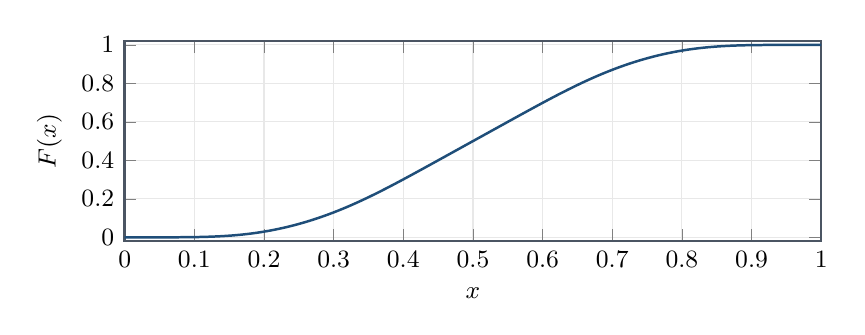
\begin{tikzpicture}
\begin{axis}[
  width=0.86\textwidth,height=0.34\textwidth,
  xmin=0,xmax=1,ymin=-0.02,ymax=1.02,
  xlabel={$x$},ylabel={$F(x)$},
  grid=major,major grid style={draw=gray!18},
  axis line style={draw=FabiusGray},
  tick label style={font=\small},label style={font=\small},
  line width=0.9pt]
\addplot[draw=FabiusBlue,smooth] coordinates {
(0,0) (0.00390625,2.29530318063e-15) (0.0078125,3.24267778096e-12) (0.01171875,1.55724628388e-10)
(0.015625,2.05217563304e-09) (0.01953125,1.37672915016e-08) (0.0234375,6.11679102547e-08) (0.02734375,2.06403160624e-07)
(0.03125,5.72675540123e-07) (0.03515625,1.37273727882e-06) (0.0390625,2.93854989634e-06) (0.04296875,5.75094375884e-06)
(0.046875,1.04681144428e-05) (0.05078125,1.79503938131e-05) (0.0546875,2.92787401716e-05) (0.05859375,4.57660504306e-05)
(0.0625,6.8962191358e-05) (0.06640625,0.00010065530553) (0.0703125,0.000142871947637) (0.07421875,0.000197876948175)
(0.078125,0.000268172107498) (0.08203125,0.00035649116457) (0.0859375,0.000465788484792) (0.08984375,0.000599220569853)
(0.09375,0.000760121286651) (0.09765625,0.000951973370934) (0.1015625,0.00117837876774) (0.10546875,0.00144302897183)
(0.109375,0.00174967653134) (0.11328125,0.00210211027671) (0.1171875,0.0025041368305) (0.12109375,0.00295956929525)
(0.125,0.00347222222222) (0.12890625,0.00404591030544) (0.1328125,0.00468444823894) (0.13671875,0.00539165057398)
(0.140625,0.0061713304131) (0.14453125,0.00702729437887) (0.1484375,0.00796333130171) (0.15234375,0.00898319372976)
(0.15625,0.0100905731578) (0.16015625,0.0112890715308) (0.1640625,0.0125821715847) (0.16796875,0.0139732071861)
(0.171875,0.0154653348369) (0.17578125,0.0170615089025) (0.1796875,0.0187644631218) (0.18359375,0.0205766992952)
(0.1875,0.0225004822531) (0.19140625,0.0245378385503) (0.1953125,0.0266905563293) (0.19921875,0.0289601854569)
(0.203125,0.03134803883) (0.20703125,0.0338551974069) (0.2109375,0.0364825215195) (0.21484375,0.0392306693634)
(0.21875,0.0421001217689) (0.22265625,0.0450912106975) (0.2265625,0.0482041489015) (0.23046875,0.0514390595834)
(0.234375,0.0547960048923) (0.23828125,0.058275010695) (0.2421875,0.0618760850662) (0.24609375,0.0655992296007)
(0.25,0.0694444444444) (0.25390625,0.0734117296007) (0.2578125,0.0775010850662) (0.26171875,0.081712510695)
(0.265625,0.0860460048923) (0.26953125,0.0905015595834) (0.2734375,0.0950791489015) (0.27734375,0.0997787106975)
(0.28125,0.104600121769) (0.28515625,0.109543169363) (0.2890625,0.11460752152) (0.29296875,0.119792697407)
(0.296875,0.12509803883) (0.30078125,0.130522685457) (0.3046875,0.136065556329) (0.30859375,0.14172533855)
(0.3125,0.147500482253) (0.31640625,0.153389199295) (0.3203125,0.159389463122) (0.32421875,0.165499008903)
(0.328125,0.171715334837) (0.33203125,0.178035707186) (0.3359375,0.184457171585) (0.33984375,0.190976571531)
(0.34375,0.197590573158) (0.34765625,0.20429569373) (0.3515625,0.211088331302) (0.35546875,0.217964794379)
(0.359375,0.224921330413) (0.36328125,0.231954150574) (0.3671875,0.239059448239) (0.37109375,0.246233410305)
(0.375,0.253472222222) (0.37890625,0.260772069295) (0.3828125,0.26812913683) (0.38671875,0.275539610277)
(0.390625,0.282999676531) (0.39453125,0.290505528972) (0.3984375,0.298053378768) (0.40234375,0.305639473371)
(0.40625,0.313260121287) (0.41015625,0.32091172057) (0.4140625,0.328590788485) (0.41796875,0.336293991165)
(0.421875,0.344018172107) (0.42578125,0.351760376948) (0.4296875,0.359517871948) (0.43359375,0.367288155306)
(0.4375,0.375068962191) (0.44140625,0.38285826605) (0.4453125,0.39065427874) (0.44921875,0.398455450394)
(0.453125,0.406260468114) (0.45703125,0.414068250944) (0.4609375,0.42187793855) (0.46484375,0.429688872737)
(0.46875,0.437500572676) (0.47265625,0.445312706403) (0.4765625,0.453125061168) (0.48046875,0.460937513767)
(0.484375,0.468750002052) (0.48828125,0.476562500156) (0.4921875,0.484375000003) (0.49609375,0.4921875)
(0.5,0.5) (0.50390625,0.5078125) (0.5078125,0.515624999997) (0.51171875,0.523437499844)
(0.515625,0.531249997948) (0.51953125,0.539062486233) (0.5234375,0.546874938832) (0.52734375,0.554687293597)
(0.53125,0.562499427324) (0.53515625,0.570311127263) (0.5390625,0.57812206145) (0.54296875,0.585931749056)
(0.546875,0.593739531886) (0.55078125,0.601544549606) (0.5546875,0.60934572126) (0.55859375,0.61714173395)
(0.5625,0.624931037809) (0.56640625,0.632711844694) (0.5703125,0.640482128052) (0.57421875,0.648239623052)
(0.578125,0.655981827893) (0.58203125,0.663706008835) (0.5859375,0.671409211515) (0.58984375,0.67908827943)
(0.59375,0.686739878713) (0.59765625,0.694360526629) (0.6015625,0.701946621232) (0.60546875,0.709494471028)
(0.609375,0.717000323469) (0.61328125,0.724460389723) (0.6171875,0.73187086317) (0.62109375,0.739227930705)
(0.625,0.746527777778) (0.62890625,0.753766589695) (0.6328125,0.760940551761) (0.63671875,0.768045849426)
(0.640625,0.775078669587) (0.64453125,0.782035205621) (0.6484375,0.788911668698) (0.65234375,0.79570430627)
(0.65625,0.802409426842) (0.66015625,0.809023428469) (0.6640625,0.815542828415) (0.66796875,0.821964292814)
(0.671875,0.828284665163) (0.67578125,0.834500991097) (0.6796875,0.840610536878) (0.68359375,0.846610800705)
(0.6875,0.852499517747) (0.69140625,0.85827466145) (0.6953125,0.863934443671) (0.69921875,0.869477314543)
(0.703125,0.87490196117) (0.70703125,0.880207302593) (0.7109375,0.88539247848) (0.71484375,0.890456830637)
(0.71875,0.895399878231) (0.72265625,0.900221289302) (0.7265625,0.904920851098) (0.73046875,0.909498440417)
(0.734375,0.913953995108) (0.73828125,0.918287489305) (0.7421875,0.922498914934) (0.74609375,0.926588270399)
(0.75,0.930555555556) (0.75390625,0.934400770399) (0.7578125,0.938123914934) (0.76171875,0.941724989305)
(0.765625,0.945203995108) (0.76953125,0.948560940417) (0.7734375,0.951795851098) (0.77734375,0.954908789302)
(0.78125,0.957899878231) (0.78515625,0.960769330637) (0.7890625,0.96351747848) (0.79296875,0.966144802593)
(0.796875,0.96865196117) (0.80078125,0.971039814543) (0.8046875,0.973309443671) (0.80859375,0.97546216145)
(0.8125,0.977499517747) (0.81640625,0.979423300705) (0.8203125,0.981235536878) (0.82421875,0.982938491097)
(0.828125,0.984534665163) (0.83203125,0.986026792814) (0.8359375,0.987417828415) (0.83984375,0.988710928469)
(0.84375,0.989909426842) (0.84765625,0.99101680627) (0.8515625,0.992036668698) (0.85546875,0.992972705621)
(0.859375,0.993828669587) (0.86328125,0.994608349426) (0.8671875,0.995315551761) (0.87109375,0.995954089695)
(0.875,0.996527777778) (0.87890625,0.997040430705) (0.8828125,0.99749586317) (0.88671875,0.997897889723)
(0.890625,0.998250323469) (0.89453125,0.998556971028) (0.8984375,0.998821621232) (0.90234375,0.999048026629)
(0.90625,0.999239878713) (0.91015625,0.99940077943) (0.9140625,0.999534211515) (0.91796875,0.999643508835)
(0.921875,0.999731827893) (0.92578125,0.999802123052) (0.9296875,0.999857128052) (0.93359375,0.999899344694)
(0.9375,0.999931037809) (0.94140625,0.99995423395) (0.9453125,0.99997072126) (0.94921875,0.999982049606)
(0.953125,0.999989531886) (0.95703125,0.999994249056) (0.9609375,0.99999706145) (0.96484375,0.999998627263)
(0.96875,0.999999427324) (0.97265625,0.999999793597) (0.9765625,0.999999938832) (0.98046875,0.999999986233)
(0.984375,0.999999997948) (0.98828125,0.999999999844) (0.9921875,0.999999999997) (0.99609375,1)
(1,1)
};
\end{axis}
\end{tikzpicture}
\caption{The bounded Fabius function on $[0,1]$.}
\label{fig:F-plot}
\end{figure}

\begin{figure}[htbp]
\centering
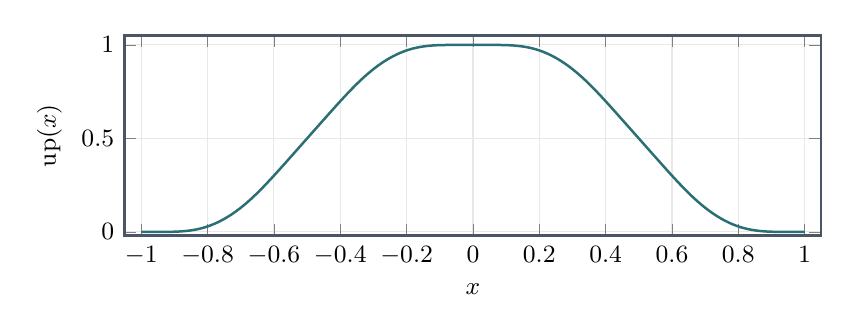
\begin{tikzpicture}
\begin{axis}[
  width=0.86\textwidth,height=0.34\textwidth,
  xmin=-1.05,xmax=1.05,ymin=-0.02,ymax=1.05,
  xlabel={$x$},ylabel={$\upf(x)$},
  grid=major,major grid style={draw=gray!18},
  axis line style={draw=FabiusGray},
  tick label style={font=\small},label style={font=\small},
  line width=0.9pt]
\addplot[draw=FabiusTeal,smooth] coordinates {
(-1,0) (-0.99609375,2.29530318063e-15) (-0.9921875,3.24267778096e-12) (-0.98828125,1.55724628388e-10)
(-0.984375,2.05217563304e-09) (-0.98046875,1.37672915016e-08) (-0.9765625,6.11679102547e-08) (-0.97265625,2.06403160624e-07)
(-0.96875,5.72675540123e-07) (-0.96484375,1.37273727882e-06) (-0.9609375,2.93854989634e-06) (-0.95703125,5.75094375884e-06)
(-0.953125,1.04681144428e-05) (-0.94921875,1.79503938131e-05) (-0.9453125,2.92787401716e-05) (-0.94140625,4.57660504306e-05)
(-0.9375,6.8962191358e-05) (-0.93359375,0.00010065530553) (-0.9296875,0.000142871947637) (-0.92578125,0.000197876948175)
(-0.921875,0.000268172107498) (-0.91796875,0.00035649116457) (-0.9140625,0.000465788484792) (-0.91015625,0.000599220569853)
(-0.90625,0.000760121286651) (-0.90234375,0.000951973370934) (-0.8984375,0.00117837876774) (-0.89453125,0.00144302897183)
(-0.890625,0.00174967653134) (-0.88671875,0.00210211027671) (-0.8828125,0.0025041368305) (-0.87890625,0.00295956929525)
(-0.875,0.00347222222222) (-0.87109375,0.00404591030544) (-0.8671875,0.00468444823894) (-0.86328125,0.00539165057398)
(-0.859375,0.0061713304131) (-0.85546875,0.00702729437887) (-0.8515625,0.00796333130171) (-0.84765625,0.00898319372976)
(-0.84375,0.0100905731578) (-0.83984375,0.0112890715308) (-0.8359375,0.0125821715847) (-0.83203125,0.0139732071861)
(-0.828125,0.0154653348369) (-0.82421875,0.0170615089025) (-0.8203125,0.0187644631218) (-0.81640625,0.0205766992952)
(-0.8125,0.0225004822531) (-0.80859375,0.0245378385503) (-0.8046875,0.0266905563293) (-0.80078125,0.0289601854569)
(-0.796875,0.03134803883) (-0.79296875,0.0338551974069) (-0.7890625,0.0364825215195) (-0.78515625,0.0392306693634)
(-0.78125,0.0421001217689) (-0.77734375,0.0450912106975) (-0.7734375,0.0482041489015) (-0.76953125,0.0514390595834)
(-0.765625,0.0547960048923) (-0.76171875,0.058275010695) (-0.7578125,0.0618760850662) (-0.75390625,0.0655992296007)
(-0.75,0.0694444444444) (-0.74609375,0.0734117296007) (-0.7421875,0.0775010850662) (-0.73828125,0.081712510695)
(-0.734375,0.0860460048923) (-0.73046875,0.0905015595834) (-0.7265625,0.0950791489015) (-0.72265625,0.0997787106975)
(-0.71875,0.104600121769) (-0.71484375,0.109543169363) (-0.7109375,0.11460752152) (-0.70703125,0.119792697407)
(-0.703125,0.12509803883) (-0.69921875,0.130522685457) (-0.6953125,0.136065556329) (-0.69140625,0.14172533855)
(-0.6875,0.147500482253) (-0.68359375,0.153389199295) (-0.6796875,0.159389463122) (-0.67578125,0.165499008903)
(-0.671875,0.171715334837) (-0.66796875,0.178035707186) (-0.6640625,0.184457171585) (-0.66015625,0.190976571531)
(-0.65625,0.197590573158) (-0.65234375,0.20429569373) (-0.6484375,0.211088331302) (-0.64453125,0.217964794379)
(-0.640625,0.224921330413) (-0.63671875,0.231954150574) (-0.6328125,0.239059448239) (-0.62890625,0.246233410305)
(-0.625,0.253472222222) (-0.62109375,0.260772069295) (-0.6171875,0.26812913683) (-0.61328125,0.275539610277)
(-0.609375,0.282999676531) (-0.60546875,0.290505528972) (-0.6015625,0.298053378768) (-0.59765625,0.305639473371)
(-0.59375,0.313260121287) (-0.58984375,0.32091172057) (-0.5859375,0.328590788485) (-0.58203125,0.336293991165)
(-0.578125,0.344018172107) (-0.57421875,0.351760376948) (-0.5703125,0.359517871948) (-0.56640625,0.367288155306)
(-0.5625,0.375068962191) (-0.55859375,0.38285826605) (-0.5546875,0.39065427874) (-0.55078125,0.398455450394)
(-0.546875,0.406260468114) (-0.54296875,0.414068250944) (-0.5390625,0.42187793855) (-0.53515625,0.429688872737)
(-0.53125,0.437500572676) (-0.52734375,0.445312706403) (-0.5234375,0.453125061168) (-0.51953125,0.460937513767)
(-0.515625,0.468750002052) (-0.51171875,0.476562500156) (-0.5078125,0.484375000003) (-0.50390625,0.4921875)
(-0.5,0.5) (-0.49609375,0.5078125) (-0.4921875,0.515624999997) (-0.48828125,0.523437499844)
(-0.484375,0.531249997948) (-0.48046875,0.539062486233) (-0.4765625,0.546874938832) (-0.47265625,0.554687293597)
(-0.46875,0.562499427324) (-0.46484375,0.570311127263) (-0.4609375,0.57812206145) (-0.45703125,0.585931749056)
(-0.453125,0.593739531886) (-0.44921875,0.601544549606) (-0.4453125,0.60934572126) (-0.44140625,0.61714173395)
(-0.4375,0.624931037809) (-0.43359375,0.632711844694) (-0.4296875,0.640482128052) (-0.42578125,0.648239623052)
(-0.421875,0.655981827893) (-0.41796875,0.663706008835) (-0.4140625,0.671409211515) (-0.41015625,0.67908827943)
(-0.40625,0.686739878713) (-0.40234375,0.694360526629) (-0.3984375,0.701946621232) (-0.39453125,0.709494471028)
(-0.390625,0.717000323469) (-0.38671875,0.724460389723) (-0.3828125,0.73187086317) (-0.37890625,0.739227930705)
(-0.375,0.746527777778) (-0.37109375,0.753766589695) (-0.3671875,0.760940551761) (-0.36328125,0.768045849426)
(-0.359375,0.775078669587) (-0.35546875,0.782035205621) (-0.3515625,0.788911668698) (-0.34765625,0.79570430627)
(-0.34375,0.802409426842) (-0.33984375,0.809023428469) (-0.3359375,0.815542828415) (-0.33203125,0.821964292814)
(-0.328125,0.828284665163) (-0.32421875,0.834500991097) (-0.3203125,0.840610536878) (-0.31640625,0.846610800705)
(-0.3125,0.852499517747) (-0.30859375,0.85827466145) (-0.3046875,0.863934443671) (-0.30078125,0.869477314543)
(-0.296875,0.87490196117) (-0.29296875,0.880207302593) (-0.2890625,0.88539247848) (-0.28515625,0.890456830637)
(-0.28125,0.895399878231) (-0.27734375,0.900221289302) (-0.2734375,0.904920851098) (-0.26953125,0.909498440417)
(-0.265625,0.913953995108) (-0.26171875,0.918287489305) (-0.2578125,0.922498914934) (-0.25390625,0.926588270399)
(-0.25,0.930555555556) (-0.24609375,0.934400770399) (-0.2421875,0.938123914934) (-0.23828125,0.941724989305)
(-0.234375,0.945203995108) (-0.23046875,0.948560940417) (-0.2265625,0.951795851098) (-0.22265625,0.954908789302)
(-0.21875,0.957899878231) (-0.21484375,0.960769330637) (-0.2109375,0.96351747848) (-0.20703125,0.966144802593)
(-0.203125,0.96865196117) (-0.19921875,0.971039814543) (-0.1953125,0.973309443671) (-0.19140625,0.97546216145)
(-0.1875,0.977499517747) (-0.18359375,0.979423300705) (-0.1796875,0.981235536878) (-0.17578125,0.982938491097)
(-0.171875,0.984534665163) (-0.16796875,0.986026792814) (-0.1640625,0.987417828415) (-0.16015625,0.988710928469)
(-0.15625,0.989909426842) (-0.15234375,0.99101680627) (-0.1484375,0.992036668698) (-0.14453125,0.992972705621)
(-0.140625,0.993828669587) (-0.13671875,0.994608349426) (-0.1328125,0.995315551761) (-0.12890625,0.995954089695)
(-0.125,0.996527777778) (-0.12109375,0.997040430705) (-0.1171875,0.99749586317) (-0.11328125,0.997897889723)
(-0.109375,0.998250323469) (-0.10546875,0.998556971028) (-0.1015625,0.998821621232) (-0.09765625,0.999048026629)
(-0.09375,0.999239878713) (-0.08984375,0.99940077943) (-0.0859375,0.999534211515) (-0.08203125,0.999643508835)
(-0.078125,0.999731827893) (-0.07421875,0.999802123052) (-0.0703125,0.999857128052) (-0.06640625,0.999899344694)
(-0.0625,0.999931037809) (-0.05859375,0.99995423395) (-0.0546875,0.99997072126) (-0.05078125,0.999982049606)
(-0.046875,0.999989531886) (-0.04296875,0.999994249056) (-0.0390625,0.99999706145) (-0.03515625,0.999998627263)
(-0.03125,0.999999427324) (-0.02734375,0.999999793597) (-0.0234375,0.999999938832) (-0.01953125,0.999999986233)
(-0.015625,0.999999997948) (-0.01171875,0.999999999844) (-0.0078125,0.999999999997) (-0.00390625,1)
(0,1) (0.00390625,1) (0.0078125,0.999999999997) (0.01171875,0.999999999844)
(0.015625,0.999999997948) (0.01953125,0.999999986233) (0.0234375,0.999999938832) (0.02734375,0.999999793597)
(0.03125,0.999999427324) (0.03515625,0.999998627263) (0.0390625,0.99999706145) (0.04296875,0.999994249056)
(0.046875,0.999989531886) (0.05078125,0.999982049606) (0.0546875,0.99997072126) (0.05859375,0.99995423395)
(0.0625,0.999931037809) (0.06640625,0.999899344694) (0.0703125,0.999857128052) (0.07421875,0.999802123052)
(0.078125,0.999731827893) (0.08203125,0.999643508835) (0.0859375,0.999534211515) (0.08984375,0.99940077943)
(0.09375,0.999239878713) (0.09765625,0.999048026629) (0.1015625,0.998821621232) (0.10546875,0.998556971028)
(0.109375,0.998250323469) (0.11328125,0.997897889723) (0.1171875,0.99749586317) (0.12109375,0.997040430705)
(0.125,0.996527777778) (0.12890625,0.995954089695) (0.1328125,0.995315551761) (0.13671875,0.994608349426)
(0.140625,0.993828669587) (0.14453125,0.992972705621) (0.1484375,0.992036668698) (0.15234375,0.99101680627)
(0.15625,0.989909426842) (0.16015625,0.988710928469) (0.1640625,0.987417828415) (0.16796875,0.986026792814)
(0.171875,0.984534665163) (0.17578125,0.982938491097) (0.1796875,0.981235536878) (0.18359375,0.979423300705)
(0.1875,0.977499517747) (0.19140625,0.97546216145) (0.1953125,0.973309443671) (0.19921875,0.971039814543)
(0.203125,0.96865196117) (0.20703125,0.966144802593) (0.2109375,0.96351747848) (0.21484375,0.960769330637)
(0.21875,0.957899878231) (0.22265625,0.954908789302) (0.2265625,0.951795851098) (0.23046875,0.948560940417)
(0.234375,0.945203995108) (0.23828125,0.941724989305) (0.2421875,0.938123914934) (0.24609375,0.934400770399)
(0.25,0.930555555556) (0.25390625,0.926588270399) (0.2578125,0.922498914934) (0.26171875,0.918287489305)
(0.265625,0.913953995108) (0.26953125,0.909498440417) (0.2734375,0.904920851098) (0.27734375,0.900221289302)
(0.28125,0.895399878231) (0.28515625,0.890456830637) (0.2890625,0.88539247848) (0.29296875,0.880207302593)
(0.296875,0.87490196117) (0.30078125,0.869477314543) (0.3046875,0.863934443671) (0.30859375,0.85827466145)
(0.3125,0.852499517747) (0.31640625,0.846610800705) (0.3203125,0.840610536878) (0.32421875,0.834500991097)
(0.328125,0.828284665163) (0.33203125,0.821964292814) (0.3359375,0.815542828415) (0.33984375,0.809023428469)
(0.34375,0.802409426842) (0.34765625,0.79570430627) (0.3515625,0.788911668698) (0.35546875,0.782035205621)
(0.359375,0.775078669587) (0.36328125,0.768045849426) (0.3671875,0.760940551761) (0.37109375,0.753766589695)
(0.375,0.746527777778) (0.37890625,0.739227930705) (0.3828125,0.73187086317) (0.38671875,0.724460389723)
(0.390625,0.717000323469) (0.39453125,0.709494471028) (0.3984375,0.701946621232) (0.40234375,0.694360526629)
(0.40625,0.686739878713) (0.41015625,0.67908827943) (0.4140625,0.671409211515) (0.41796875,0.663706008835)
(0.421875,0.655981827893) (0.42578125,0.648239623052) (0.4296875,0.640482128052) (0.43359375,0.632711844694)
(0.4375,0.624931037809) (0.44140625,0.61714173395) (0.4453125,0.60934572126) (0.44921875,0.601544549606)
(0.453125,0.593739531886) (0.45703125,0.585931749056) (0.4609375,0.57812206145) (0.46484375,0.570311127263)
(0.46875,0.562499427324) (0.47265625,0.554687293597) (0.4765625,0.546874938832) (0.48046875,0.539062486233)
(0.484375,0.531249997948) (0.48828125,0.523437499844) (0.4921875,0.515624999997) (0.49609375,0.5078125)
(0.5,0.5) (0.50390625,0.4921875) (0.5078125,0.484375000003) (0.51171875,0.476562500156)
(0.515625,0.468750002052) (0.51953125,0.460937513767) (0.5234375,0.453125061168) (0.52734375,0.445312706403)
(0.53125,0.437500572676) (0.53515625,0.429688872737) (0.5390625,0.42187793855) (0.54296875,0.414068250944)
(0.546875,0.406260468114) (0.55078125,0.398455450394) (0.5546875,0.39065427874) (0.55859375,0.38285826605)
(0.5625,0.375068962191) (0.56640625,0.367288155306) (0.5703125,0.359517871948) (0.57421875,0.351760376948)
(0.578125,0.344018172107) (0.58203125,0.336293991165) (0.5859375,0.328590788485) (0.58984375,0.32091172057)
(0.59375,0.313260121287) (0.59765625,0.305639473371) (0.6015625,0.298053378768) (0.60546875,0.290505528972)
(0.609375,0.282999676531) (0.61328125,0.275539610277) (0.6171875,0.26812913683) (0.62109375,0.260772069295)
(0.625,0.253472222222) (0.62890625,0.246233410305) (0.6328125,0.239059448239) (0.63671875,0.231954150574)
(0.640625,0.224921330413) (0.64453125,0.217964794379) (0.6484375,0.211088331302) (0.65234375,0.20429569373)
(0.65625,0.197590573158) (0.66015625,0.190976571531) (0.6640625,0.184457171585) (0.66796875,0.178035707186)
(0.671875,0.171715334837) (0.67578125,0.165499008903) (0.6796875,0.159389463122) (0.68359375,0.153389199295)
(0.6875,0.147500482253) (0.69140625,0.14172533855) (0.6953125,0.136065556329) (0.69921875,0.130522685457)
(0.703125,0.12509803883) (0.70703125,0.119792697407) (0.7109375,0.11460752152) (0.71484375,0.109543169363)
(0.71875,0.104600121769) (0.72265625,0.0997787106975) (0.7265625,0.0950791489015) (0.73046875,0.0905015595834)
(0.734375,0.0860460048923) (0.73828125,0.081712510695) (0.7421875,0.0775010850662) (0.74609375,0.0734117296007)
(0.75,0.0694444444444) (0.75390625,0.0655992296007) (0.7578125,0.0618760850662) (0.76171875,0.058275010695)
(0.765625,0.0547960048923) (0.76953125,0.0514390595834) (0.7734375,0.0482041489015) (0.77734375,0.0450912106975)
(0.78125,0.0421001217689) (0.78515625,0.0392306693634) (0.7890625,0.0364825215195) (0.79296875,0.0338551974069)
(0.796875,0.03134803883) (0.80078125,0.0289601854569) (0.8046875,0.0266905563293) (0.80859375,0.0245378385503)
(0.8125,0.0225004822531) (0.81640625,0.0205766992952) (0.8203125,0.0187644631218) (0.82421875,0.0170615089025)
(0.828125,0.0154653348369) (0.83203125,0.0139732071861) (0.8359375,0.0125821715847) (0.83984375,0.0112890715308)
(0.84375,0.0100905731578) (0.84765625,0.00898319372976) (0.8515625,0.00796333130171) (0.85546875,0.00702729437887)
(0.859375,0.0061713304131) (0.86328125,0.00539165057398) (0.8671875,0.00468444823894) (0.87109375,0.00404591030544)
(0.875,0.00347222222222) (0.87890625,0.00295956929525) (0.8828125,0.0025041368305) (0.88671875,0.00210211027671)
(0.890625,0.00174967653134) (0.89453125,0.00144302897183) (0.8984375,0.00117837876774) (0.90234375,0.000951973370934)
(0.90625,0.000760121286651) (0.91015625,0.000599220569853) (0.9140625,0.000465788484792) (0.91796875,0.00035649116457)
(0.921875,0.000268172107498) (0.92578125,0.000197876948175) (0.9296875,0.000142871947637) (0.93359375,0.00010065530553)
(0.9375,6.8962191358e-05) (0.94140625,4.57660504306e-05) (0.9453125,2.92787401716e-05) (0.94921875,1.79503938131e-05)
(0.953125,1.04681144428e-05) (0.95703125,5.75094375884e-06) (0.9609375,2.93854989634e-06) (0.96484375,1.37273727882e-06)
(0.96875,5.72675540123e-07) (0.97265625,2.06403160624e-07) (0.9765625,6.11679102547e-08) (0.98046875,1.37672915016e-08)
(0.984375,2.05217563304e-09) (0.98828125,1.55724628388e-10) (0.9921875,3.24267778096e-12) (0.99609375,2.29530318063e-15)
(1,0)
};
\end{axis}
\end{tikzpicture}
\caption{Rvachev's even compactly supported up-function.}
\label{fig:up-plot}
\end{figure}

\section{The signed global extension and differential self-similarity}

The signed extension $\Thetaf$ removes the artificial clamping at $1$.  Its
advantage is that the local equation becomes a global one with no reflected term.

\begin{theorem}[Global differential equation]\label{thm:theta-global-diff}
The function $\Thetaf$ is $C^\infty$ on $\R$ and satisfies
\begin{equation}\label{eq:theta-global-diff}
  \Thetaf'(x)=2\Thetaf(2x),\qquad x\in\R.
\end{equation}
For every $k\ge0$,
\begin{equation}\label{eq:theta-iterated-derivative}
  \Thetaf^{(k)}(x)=2^{\binom{k+1}{2}}\Thetaf(2^kx).
\end{equation}
On the support of $\upf$,
\begin{equation}\label{eq:up-derivative-theta}
  \upf^{(k)}(x)=2^{\binom{k+1}{2}}
  \Thetaf\bigl(2^k(x+1)\bigr),\qquad -1\le x\le1.
\end{equation}
\end{theorem}

\begin{proof}
Because the sum \eqref{eq:global-theta} is locally finite, it may be differentiated
term by term.  Apply \eqref{eq:rvachev-equation}:
\begin{align*}
 \Thetaf'(x)
 &=2\sum_{n\ge0}\epsTM_n
   \bigl[\upf(2x-4n-1)-\upf(2x-4n-3)\bigr]\\
 &=2\sum_{n\ge0}\epsTM_{2n}\upf(2x-2(2n)-1)
   +2\sum_{n\ge0}\epsTM_{2n+1}\upf(2x-2(2n+1)-1)\\
 &=2\Thetaf(2x),
\end{align*}
where \eqref{eq:TM-scaling} was used in the second equality.  Repeated
differentiation proves \eqref{eq:theta-iterated-derivative}: the factors accumulated
are $2^1,2^2,\ldots,2^k$, whose product is $2^{\binom{k+1}{2}}$.
On $[-1,1]$ one has $\upf(x)=\Thetaf(x+1)$; differentiating and applying
\eqref{eq:theta-iterated-derivative} gives
\eqref{eq:up-derivative-theta}.
\end{proof}

\begin{corollary}[Flat endpoints]\label{cor:flat-endpoints}
Every derivative of $F$ vanishes at $0$, and every derivative of $\upf$ vanishes at
$-1$ and $1$:
\begin{equation}\label{eq:flatness}
  F^{(k)}(0)=0,
  \qquad
  \upf^{(k)}(-1)=\upf^{(k)}(1)=0
  \qquad(k\ge0).
\end{equation}
\end{corollary}

\begin{proof}
The clamped function is identically zero to the left of $0$, so smoothness already
forces the first statement.  Alternatively, use
\eqref{eq:theta-iterated-derivative} and $\Thetaf(0)=0$.  Equation
\eqref{eq:up-derivative-theta} gives the value at $-1$ directly.  Evenness supplies
the value at $1$.
\end{proof}

The next phenomenon is one of the function's most striking features: at a dyadic
point the Taylor series is a polynomial, but the function does not equal that
polynomial in any neighborhood.

\begin{theorem}[Dyadic jets]\label{thm:dyadic-jets}
Let
\begin{equation}\label{eq:centered-dyadic}
  x_{n,a}=\frac{a-2^n}{2^n},
  \qquad 0\le a\le2^{n+1}.
\end{equation}
Then
\begin{equation}\label{eq:dyadic-high-derivatives-zero}
  \upf^{(k)}(x_{n,a})=0\qquad(k>n).
\end{equation}
If $a$ is odd, then
\begin{equation}\label{eq:dyadic-top-derivative-nonzero}
  \upf^{(n)}(x_{n,a})\ne0.
\end{equation}
Hence the formal Taylor polynomial at a reduced level-$n$ dyadic point has degree
exactly $n$.
\end{theorem}

\begin{proof}
By \eqref{eq:up-derivative-theta},
\[
 \upf^{(k)}(x_{n,a})
 =2^{\binom{k+1}{2}}\Thetaf\left(2^k\frac{a}{2^n}\right).
\]
If $k>n$, the argument is the even integer $2^{k-n}a$.  Formula
\eqref{eq:theta-band} shows that $\Thetaf$ vanishes at every even nonnegative
integer, because these points are support endpoints of the translated bumps.
This proves \eqref{eq:dyadic-high-derivatives-zero}.  When $k=n$ and $a$ is odd,
write $a=2m+1$.  Then
$\Thetaf(a)=\epsTM_m\upf(0)=\epsTM_m\ne0$, proving
\eqref{eq:dyadic-top-derivative-nonzero}.
\end{proof}

\begin{theorem}[Failure of analyticity on the support]\label{thm:nowhere-analytic}
The function $\upf$ is not real analytic at any point of $[-1,1]$.  Consequently
$F$ is not real analytic at any point of $[0,1]$.
\end{theorem}

\begin{proof}
Reduced dyadic points of arbitrarily high level are dense in $[-1,1]$.  Suppose
$\upf$ were analytic at some $x$ in the support.  It would then be analytic on a
small open interval $I$ around $x$.  Choose a reduced dyadic $y=x_{n,a}\in I$.
By \cref{thm:dyadic-jets}, all derivatives of order greater than $n$ vanish at $y$,
so the analytic Taylor series at $y$ is a polynomial of degree at most $n$.
Therefore $\upf$ agrees with a polynomial on a neighborhood of $y$.

Choose inside that neighborhood another reduced dyadic point $z$ of level $m>n$.
The same polynomial has zero $m$-th derivative, whereas
\eqref{eq:dyadic-top-derivative-nonzero} says $\upf^{(m)}(z)\ne0$.  This
contradiction proves the claim.  The bridge between $F$ and $\upf$ transfers the
statement to $[0,1]$.
\end{proof}

\begin{remark}
There is no contradiction with the fact that $\upf$ is analytic on
$(-\infty,-1)$ and $(1,\infty)$: it is identically zero there.  The theorem is
precisely a statement about every point of the topological support.
\end{remark}

\section{Fourier analysis, infinite products, and Poisson summation}\label{sec:fourier}

\subsection{The entire Fourier transform}

We now collect the Fourier statements used implicitly above.  Our convention is
\begin{equation}\label{eq:Fourier-convention}
  \widehat g(z)=\int_{\R}g(x)e^{-2\pi\ii xz}\dd x.
\end{equation}
Because $\upf\in C_c^\infty(\R)$, its transform is entire and rapidly decreasing
on every horizontal strip.  The refinement equation determines it exactly.

\begin{theorem}[Sinc product and inversion]\label{thm:Fourier-product-inversion}
For every $z\in\C$,
\begin{equation}\label{eq:Fourier-product-main}
  \Fourier(z)=\prod_{j=0}^{\infty}
  \frac{\sin(\pi z/2^j)}{\pi z/2^j}.
\end{equation}
For every $x\in\R$,
\begin{equation}\label{eq:Fourier-inversion-main}
  \upf(x)=\int_{\R}\Fourier(t)e^{2\pi\ii tx}\dd t.
\end{equation}
The product and all of its complex derivatives converge locally uniformly.
\end{theorem}

\begin{proof}
The product identity is \eqref{eq:up-Fourier-product}, with
$\widehat{\upf}(0)=\int\upf=1$.  Local uniform convergence follows from
$1-\sinc z=O(z^2)$ and the convergence of $\sum4^{-j}$, uniformly on compact
sets.  Since $\Fourier$ is integrable by \cref{lem:Phi-Schwartz}, ordinary Fourier
inversion applies.  The same decay after multiplication by powers of $t$ justifies
differentiation under the inversion integral to every order.
\end{proof}

The first factor already shows that
\begin{equation}\label{eq:integer-zeros}
  \Fourier(m)=0\qquad(m\in\Z\setminus\{0\}).
\end{equation}
The zero multiplicities contain additional arithmetic information.  If
$m\ne0$ is an integer and $\nu_2(m)$ is its $2$-adic valuation, then exactly the
factors with $0\le j\le\nu_2(m)$ vanish, so
\begin{equation}\label{eq:Fourier-zero-order}
  \ord_{z=m}\Fourier(z)=1+\nu_2(m).
\end{equation}
This leads to a third entire product.

\begin{theorem}[Three equivalent products]\label{thm:three-products}
The following ordered products agree for every $z\in\C$:
\begin{align}
  \Fourier(z)
  &=\prod_{j=0}^{\infty}\sinc\left(\frac{\pi z}{2^j}\right),
    \label{eq:product-sinc}\\
  &=\prod_{m=1}^{\infty}
    \left(\cos\frac{\pi z}{2^m}\right)^m,
    \label{eq:product-cos}\\
  &=\prod_{m=1}^{\infty}
    \left(1-\frac{z^2}{m^2}\right)^{1+\nu_2(m)}.
    \label{eq:product-zero}
\end{align}
The last product is understood in its natural symmetric canonical ordering.
\end{theorem}

\begin{proof}
The elementary identity
\begin{equation}\label{eq:sinc-half}
  \sinc z=\cos(z/2)\sinc(z/2)
\end{equation}
implies, for the first $N$ sinc factors,
\begin{equation}\label{eq:finite-cos-telescope}
  \prod_{j=0}^{N-1}\sinc\left(\frac{\pi z}{2^j}\right)
  =\left[\prod_{m=1}^{N}
    \left(\cos\frac{\pi z}{2^m}\right)^m\right]
    \sinc\left(\frac{\pi z}{2^N}\right)^N.
\end{equation}
The final factor tends to $1$ locally uniformly, since
$N(1-\sinc(\pi z/2^N))=O(N4^{-N})$.  This proves
\eqref{eq:product-cos}.

For \eqref{eq:product-zero}, use the Weierstrass product
$\sinc(\pi z)=\prod_{r\ge1}(1-z^2/r^2)$ in each sinc factor.  A zero at the
integer $m$ occurs in the $j$-th scaled factor precisely when $2^j\mid m$.
Thus its total multiplicity is $1+\nu_2(m)$, as in
\eqref{eq:Fourier-zero-order}.  Regrouping symmetric pairs of zeros gives the
stated canonical product.
\end{proof}

\subsection{Poisson summation and partition of unity}

Since $\upf$ is a compactly supported smooth function, both it and its transform
are Schwartz functions.  Poisson summation is therefore available without any
conditional convergence issue.

\begin{theorem}[Poisson summation]\label{thm:poisson}
For $a>0$ and $x\in\R$,
\begin{equation}\label{eq:poisson-general}
  \sum_{m\in\Z}\upf(x+am)
  =\frac1a\sum_{k\in\Z}\Fourier(k/a)e^{2\pi\ii kx/a}.
\end{equation}
Both series converge absolutely and locally uniformly with all derivatives.
\end{theorem}

\begin{proof}
Apply the standard Poisson formula to the Schwartz function
$t\mapsto\upf(x+at)$.  The scaling and translation rules for the Fourier transform
give \eqref{eq:poisson-general}.  Rapid decay gives the asserted convergence.
\end{proof}

The integer zeros \eqref{eq:integer-zeros} collapse several specializations.

\begin{corollary}[Integer translates]\label{cor:partition-unity}
For all $x\in\R$,
\begin{equation}\label{eq:partition-unity}
  \sum_{m\in\Z}\upf(x+m)=1.
\end{equation}
In particular, for $0\le x\le1$,
\begin{equation}\label{eq:two-term-partition}
  \upf(x)+\upf(x-1)=1.
\end{equation}
More generally, for every positive integer $n$,
\begin{equation}\label{eq:n-partition}
  \sum_{m\in\Z}\upf\left(x+\frac{m}{n}\right)=n.
\end{equation}
\end{corollary}

\begin{proof}
Set $a=1$ in \eqref{eq:poisson-general}; only $k=0$ survives.  Support reduces the
left side to two terms on $[0,1]$.  For \eqref{eq:n-partition}, set $a=1/n$;
the dual samples are at $kn$, again nonzero integers unless $k=0$.
\end{proof}

The identity \eqref{eq:two-term-partition} is exactly the Fabius symmetry in up
coordinates: $\upf(x-1)=F(x)$ and $\upf(x)=1-F(x)$.

Taking lattice spacing $2$ instead gives the rapidly convergent cosine expansion.

\begin{corollary}[Cosine expansion]\label{cor:cosine-expansion}
For $|x|\le1$,
\begin{equation}\label{eq:up-cosine-series}
  \upf(x)=\frac12+
  \sum_{k=0}^{\infty}
  \Fourier\left(\frac{2k+1}{2}\right)
  \cos\bigl((2k+1)\pi x\bigr).
\end{equation}
The series and all of its derivatives converge uniformly.
\end{corollary}

\begin{proof}
For $|x|\le1$, support makes
$\sum_m\upf(x+2m)=\upf(x)$.  In the dual series, every nonzero even index samples
$\Fourier$ at a nonzero integer and vanishes.  Pair the terms indexed by
$2k+1$ and $-(2k+1)$, using that $\Fourier$ is real and even on the real axis.
Rapid decay proves smooth uniform convergence.
\end{proof}

\subsection{A useful sampling identity}

At $x=0$, \eqref{eq:poisson-general} reads
\begin{equation}\label{eq:poisson-at-zero}
  \sum_{m\in\Z}\upf(am)
  =\frac1a\sum_{m\in\Z}\Fourier(m/a).
\end{equation}
When $1/2\le a\le1$, only the samples $0,\pm a$ of $\upf$ can be nonzero, so
\begin{equation}\label{eq:sampling-a}
  1+2\upf(a)=\frac1a\sum_{m\in\Z}\Fourier(m/a).
\end{equation}
Equivalently,
$a+2a\upf(a)=\sum_m\Fourier(m/a)$.  This is one of several ways to turn values
of the bump into rapidly convergent transform sums.

\section{Moments and generating functions}\label{sec:moments}

Two rational moment sequences organize much of the exact arithmetic.

\begin{definition}[Even moments]\label{def:c-moments}
For $n\ge0$, let
\begin{equation}\label{eq:c-moment-def}
  c_n=\int_{\R}x^{2n}\upf(x)\dd x.
\end{equation}
All odd moments vanish because $\upf$ is even.
\end{definition}

\begin{definition}[Half-moments]\label{def:d-moments}
Let $d_0=1$, and for $n\ge1$ put
\begin{equation}\label{eq:d-half-moment-def}
  d_n=n\int_0^1x^{n-1}\upf(x)\dd x.
\end{equation}
\end{definition}

\subsection{The moment series and the recurrence for \texorpdfstring{$c_n$}{c n}}

Expanding the Fourier integral at the origin gives
\begin{equation}\label{eq:moment-series}
  \Fourier(z)=\sum_{n=0}^{\infty}(-1)^n
  \frac{c_n}{(2n)!}(2\pi z)^{2n}.
\end{equation}
The series is entire because $\Fourier$ is entire.

\begin{theorem}[Moment recurrence]\label{thm:c-recurrence}
The moments are positive rational numbers satisfying
\begin{equation}\label{eq:c-recurrence}
  c_0=1,
  \qquad
  (2n+1)(2^{2n}-1)c_n
  =\sum_{k=0}^{n-1}\binom{2n+1}{2k}c_k
  \quad(n\ge1).
\end{equation}
\end{theorem}

\begin{proof}
The Fourier refinement equation is
\begin{equation}\label{eq:Fourier-refinement}
  \Fourier(z)=\sinc(\pi z)\Fourier(z/2).
\end{equation}
Insert the power series for $\sinc(\pi z)$ and
\eqref{eq:moment-series}, then compare the coefficient of $z^{2n}$.  One obtains
\begin{equation}\label{eq:c-pre-recurrence}
  (2n+1)2^{2n}c_n=
  \sum_{k=0}^{n}\binom{2n+1}{2k}c_k.
\end{equation}
The last summand is $(2n+1)c_n$; moving it to the left gives
\eqref{eq:c-recurrence}.  Positivity follows either from the integral definition or
inductively from the recurrence, and rationality follows inductively because the
coefficients are integers.
\end{proof}

The first values are
\begin{equation}\label{eq:first-c-values}
\begin{split}
 c_0&=1,\qquad c_1=\frac19,\qquad c_2=\frac{19}{675},
 \qquad c_3=\frac{583}{59535},\\
 c_4&=\frac{132809}{32531625},\qquad
 c_5=\frac{46840699}{24405225075},\quad\ldots
\end{split}
\end{equation}

\subsection{The exponential generating function and the \texorpdfstring{$d_n$}{d n} recurrence}

Define
\begin{equation}\label{eq:f-generating}
  f(z)=1+z\int_0^1\upf(t)e^{zt}\dd t.
\end{equation}
There are three equivalent interpretations:
\begin{equation}\label{eq:f-three-forms}
  f(z)=\E(e^{zX})
  =e^{z/2}\Fourier\left(\frac{\ii z}{4\pi}\right)
  =\sum_{n=0}^{\infty}\frac{d_n}{n!}z^n.
\end{equation}
The first equality follows by integration by parts and
$F(t)=1-\upf(t)$ on $[0,1]$; the second follows from $X=(Y+1)/2$; the third is the
definition of the Taylor coefficients and agrees with
\eqref{eq:d-half-moment-def}.

Split the random series as $X=U_1/2+X'/2$, with $X'$ an independent copy of $X$.
Its moment generating function obeys
\begin{equation}\label{eq:f-functional}
  f(2z)=\frac{e^z-1}{z}f(z),
\end{equation}
where the quotient is assigned its removable value $1$ at $z=0$.

\begin{theorem}[Half-moment recurrence]\label{thm:d-recurrence}
The half-moments satisfy
\begin{equation}\label{eq:d-recurrence}
  d_0=1,
  \qquad
  (n+1)(2^n-1)d_n
  =\sum_{k=0}^{n-1}\binom{n+1}{k}d_k
  \quad(n\ge1).
\end{equation}
\end{theorem}

\begin{proof}
Multiply \eqref{eq:f-functional} by $z$:
$zf(2z)=(e^z-1)f(z)$.  Substitute the exponential generating series and compare
the coefficient of $z^{n+1}$.  The term containing $d_n$ appears on both sides;
collecting it gives \eqref{eq:d-recurrence}.
\end{proof}

The first values are
\begin{equation}\label{eq:first-d-values}
  1,\ \frac12,\ \frac5{18},\ \frac16,\ \frac{143}{1350},
  \frac{19}{270},\ \frac{1153}{23814},\ \frac{583}{17010},
  \frac{1616353}{65063250},\ldots
\end{equation}

\subsection{Relations between the two moment systems}

\begin{theorem}[Binomial transform]\label{thm:d-from-c}
For every $n\ge0$,
\begin{equation}\label{eq:d-from-c}
  d_n=2^{-n}\sum_{k=0}^{\floor{n/2}}\binom{n}{2k}c_k.
\end{equation}
\end{theorem}

\begin{proof}
For $n\ge1$, integrate \eqref{eq:d-half-moment-def} by parts:
\begin{align*}
 d_n
 &=\int_0^1\upf(t)\dd(t^n)
 =-\int_0^1t^n\upf'(t)\dd t\\
 &=2\int_0^1t^n\upf(2t-1)\dd t
 =\int_{-1}^1\upf(x)\left(\frac{x+1}{2}\right)^n\dd x.
\end{align*}
The boundary term vanishes because $\upf(1)=0$ and $t^n=0$ at $t=0$.
Expand $(x+1)^n$.  Odd moments vanish, while the $2k$-th moment is $c_k$.
This gives \eqref{eq:d-from-c}.  The case $n=0$ is immediate.
\end{proof}

The inverse-power values of $F$ are precisely normalized half-moments.

\begin{theorem}[Inverse powers of two]\label{thm:inverse-power-value}
For every $n\ge0$,
\begin{equation}\label{eq:inverse-power-value}
  d_n=n!\,2^{\binom n2}F(2^{-n}),
  \qquad
  F(2^{-n})=\frac{d_n}{n!\,2^{\binom n2}}.
\end{equation}
\end{theorem}

\begin{proof}
The case $n=0$ is $F(1)=d_0=1$, so suppose $n\ge1$.  On $[0,1]$ we have
$\upf(t)=F(1-t)$.  After the substitution $u=1-t$,
\begin{equation}\label{eq:dn-weighted-F}
  d_n=n\int_0^1(1-u)^{n-1}F(u)\dd u.
\end{equation}
Set $g(u)=F(u/2^n)$.  Repeated differentiation of
$F'(x)=2F(2x)$ gives, for $0\le u\le1$,
\begin{equation}\label{eq:scaled-nth-derivative}
  g^{(n)}(u)
  =2^{-n^2}F^{(n)}(u/2^n)
  =2^{-\binom n2}F(u).
\end{equation}
All derivatives of $F$ vanish at $0$, so $g^{(j)}(0)=0$ for
$0\le j<n$.  Integrating by parts $n$ times therefore yields
\begin{equation}\label{eq:beta-derivative-integral}
  \int_0^1(1-u)^{n-1}g^{(n)}(u)\dd u=(n-1)!\,g(1).
\end{equation}
Indeed, the boundary terms at $u=0$ vanish by flatness; those at $u=1$
vanish until the last integration because of the factor $(1-u)$, and the
last one is $(n-1)!g(1)$.

Substituting \eqref{eq:scaled-nth-derivative} into
\eqref{eq:dn-weighted-F} and using $g(1)=F(2^{-n})$ gives
\[
 d_n=n\,2^{\binom n2}(n-1)!\,F(2^{-n}),
\]
which is \eqref{eq:inverse-power-value}.
\end{proof}

Combining \cref{thm:d-from-c,thm:inverse-power-value} gives, for $k\ge0$,
\begin{equation}\label{eq:moment-from-inverse-F}
  c_k=2(2k)!\,2^{\binom{2k+1}{2}}F(2^{-2k-1}).
\end{equation}
This bridge will reappear in the exact dyadic formulas and in the Legendre
coefficients.

\subsection{Bernoulli recurrences}

The functional equations may also be inverted before coefficients are compared.
Using
\begin{align}
  \frac{\pi z}{\sin\pi z}
  &=1+\sum_{n\ge1}(-1)^{n+1}
  \frac{B_{2n}(2^{2n}-2)}{(2n)!}(\pi z)^{2n},
  \label{eq:Bernoulli-sin}\\
  \frac{z}{e^z-1}&=\sum_{n\ge0}\frac{B_n}{n!}z^n,
  \label{eq:Bernoulli-exp}
\end{align}
coefficient comparison gives the following equivalent recurrences.

\begin{proposition}[Bernoulli recurrences]\label{prop:Bernoulli-recurrences}
For $n\ge1$,
\begin{equation}\label{eq:c-Bernoulli}
  c_n=\frac1{2^{2n}-1}\sum_{k=1}^{n}
  2^{2n-2k}(2^{2k}-2)\binom{2n}{2k}B_{2k}c_{n-k},
\end{equation}
and
\begin{equation}\label{eq:d-Bernoulli}
  d_n=\frac{n2^{n-2}}{2^n-1}d_{n-1}
  -\frac1{2^n-1}\sum_{k=1}^{\floor{n/2}}
  \binom n{2k}2^{n-2k}B_{2k}d_{n-2k}.
\end{equation}
\end{proposition}

\begin{proof}
Rewrite \eqref{eq:Fourier-refinement} as
$(\pi z/\sin\pi z)\Fourier(z)=\Fourier(z/2)$ and
\eqref{eq:f-functional} as
$(z/(e^z-1))f(2z)=f(z)$.  Insert
\eqref{eq:Bernoulli-sin}--\eqref{eq:Bernoulli-exp}, then compare coefficients.
The odd Bernoulli numbers beyond $B_1$ vanish, producing the displayed forms.
\end{proof}

\section{Exact evaluation at dyadic rationals}\label{sec:dyadic}

Dyadic points are exceptional in two complementary ways.  Analytically, every
sufficiently high derivative vanishes there.  Arithmetically, the value is rational
and can be computed by finite exact operations.  We now prove two formulas: a
closed sum that displays the Thue--Morse and moment structure, and a recursive
formula adapted to computation.

\subsection{The closed Thue--Morse--moment formula}

\begin{theorem}[Closed dyadic formula]\label{thm:closed-dyadic}
Let $n,a\in\N$.  Then the signed global extension satisfies
\begin{equation}\label{eq:closed-dyadic}
 \Thetaf\left(\frac{a}{2^n}\right)
 =\frac{2^{-\binom{n+1}{2}}}{n!}
 \sum_{h=0}^{a-1}\epsTM_h
 \sum_{k=0}^{\floor{n/2}}
 \binom n{2k}(2a-2h-1)^{n-2k}c_k.
\end{equation}
The outer sum is empty when $a=0$.  If $0\le a\le2^n$, then
$\Thetaf(a/2^n)=F(a/2^n)$, so \eqref{eq:closed-dyadic} is an exact formula for the
bounded Fabius function.  If $-2^n\le q\le2^n$, the up-value
$\upf(q/2^n)$ is obtained by taking $a=q+2^n$.
\end{theorem}

\begin{proof}
All derivatives of $\Thetaf$ vanish at $0$.  Taylor's theorem with integral
remainder, applied through order $n$, therefore gives
\begin{equation}\label{eq:closed-proof-taylor}
 \Thetaf(x)=\frac1{n!}\int_0^x(x-t)^n\Thetaf^{(n+1)}(t)\dd t.
\end{equation}
Put $x=a/2^n$ and use \eqref{eq:theta-iterated-derivative}:
\[
 \Thetaf^{(n+1)}(t)=2^{\binom{n+2}{2}}\Thetaf(2^{n+1}t).
\]
With $u=2^{n+1}t$, equation \eqref{eq:closed-proof-taylor} becomes
\begin{equation}\label{eq:closed-proof-scaled}
 \Thetaf\left(\frac a{2^n}\right)
 =\frac{2^{-\binom{n+1}{2}}}{n!}
 \int_0^{2a}(2a-u)^n\Thetaf(u)\dd u.
\end{equation}
Split $[0,2a]$ into the bands $[2h,2h+2]$.  By
\eqref{eq:theta-band}, and with $v=u-2h-1$,
\begin{align*}
 \int_{2h}^{2h+2}(2a-u)^n\Thetaf(u)\dd u
 &=\epsTM_h\int_{-1}^{1}
   (2a-2h-1-v)^n\upf(v)\dd v\\
 &=\epsTM_h\sum_{j=0}^n\binom nj
   (2a-2h-1)^{n-j}(-1)^j
   \int_{-1}^{1}v^j\upf(v)\dd v.
\end{align*}
Odd moments vanish, and the $2k$-th moment is $c_k$.  The surviving signs are
$(-1)^{2k}=1$, producing precisely \eqref{eq:closed-dyadic}.
\end{proof}

\begin{corollary}[Rationality]\label{cor:dyadic-rationality}
The values $F(a/2^n)$ and $\upf(q/2^n)$ are rational at every dyadic point in
their respective domains.  The signed evaluator
$\Thetaf(a/2^n)$ is rational for every nonnegative integer numerator $a$.
\end{corollary}

\begin{proof}
The moments $c_k$ are rational by \cref{thm:c-recurrence}; every other quantity
in \eqref{eq:closed-dyadic} is integral or a power of $2$ divided by a factorial.
\end{proof}

The formula is closed but not necessarily the fastest computational route.  It is,
however, ideal for proving denominator bounds because the only nonintegral inputs
are the finitely many $c_k$ with $k\le\floor{n/2}$.

\subsection{A complete level-four table}

At denominator $16$, every value has common denominator $2\,073\,600$:
\begin{equation}\label{eq:level-four-common-den}
  F(a/16)=\frac{N_a}{2\,073\,600}.
\end{equation}
The exact numerators are
\begin{center}
\small
\begin{tabular}{c|rrrrrrrrr}
\toprule
$a$&0&1&2&3&4&5&6&7&8\\
\midrule
$N_a$&0&143&7\,200&46\,657&144\,000&305\,857&525\,600&777\,743&1\,036\,800\\
\bottomrule
\end{tabular}

\vspace{0.7em}
\begin{tabular}{c|rrrrrrrr}
\toprule
$a$&9&10&11&12&13&14&15&16\\
\midrule
$N_a$&1\,295\,857&1\,548\,000&1\,767\,743&1\,929\,600&2\,026\,943&2\,066\,400&2\,073\,457&2\,073\,600\\
\bottomrule
\end{tabular}
\end{center}
The symmetry $N_{16-a}=2\,073\,600-N_a$ is just
$F(1-x)=1-F(x)$.

\subsection{The inverse-power lookup table}

The first values furnished by \eqref{eq:inverse-power-value} are
\begin{center}
\begin{tabular}{ccl}
\toprule
$n$&$d_n$&$F(2^{-n})$\\
\midrule
0&$1$&$1$\\
1&$1/2$&$1/2$\\
2&$5/18$&$5/72$\\
3&$1/6$&$1/288$\\
4&$143/1350$&$143/2\,073\,600$\\
5&$19/270$&$19/33\,177\,600$\\
6&$1153/23814$&$1153/561\,842\,749\,440$\\
7&$583/17010$&$583/179\,789\,679\,820\,800$\\
\bottomrule
\end{tabular}
\end{center}
The table can be generated in $O(N^2)$ rational operations from
\eqref{eq:d-recurrence}.

\subsection{Taylor reduction by the highest binary digit}

The next formula was designed for exact evaluation.  It removes the largest power
of two present in the argument and replaces the function value by one at a smaller
argument plus a finite polynomial whose coefficients come from the lookup table.

\begin{theorem}[Taylor-block reduction]\label{thm:Taylor-reduction}
Let $x>0$, and let $n\in\Z$ be the unique integer such that
\begin{equation}\label{eq:Taylor-cell}
  2^{-n}\le x<2^{-n+1}.
\end{equation}
Put $y=x-2^{-n}$.  Then
\begin{equation}\label{eq:Taylor-reduction}
 \Thetaf(x)=-\Thetaf(y)+
 \begin{cases}
 \displaystyle
 \sum_{k=0}^{n}
 2^{\binom{k+1}{2}-\binom{n-k}{2}}
 \frac{d_{n-k}}{(n-k)!}\frac{y^k}{k!},& n\ge0,\\[3ex]
 0,&n<0.
 \end{cases}
\end{equation}
For $0<x\le1$, one always has $n\ge0$ and $\Thetaf(x)=F(x)$.
\end{theorem}

\begin{proof}
Assume first that $n\ge0$, set $a=2^{-n}$, and apply Taylor's theorem at $a$ to
order $n$:
\begin{equation}\label{eq:Taylor-at-a}
 \Thetaf(a+y)=\sum_{k=0}^n\frac{\Thetaf^{(k)}(a)}{k!}y^k
 +\frac1{n!}\int_a^{a+y}(a+y-t)^n\Thetaf^{(n+1)}(t)\dd t.
\end{equation}
The derivatives at the base point are exact inverse-power values:
\begin{align}
 \Thetaf^{(k)}(2^{-n})
 &=2^{\binom{k+1}{2}}\Thetaf(2^{k-n})\notag\\
 &=2^{\binom{k+1}{2}}
   F(2^{-(n-k)})\notag\\
 &=2^{\binom{k+1}{2}-\binom{n-k}{2}}
   \frac{d_{n-k}}{(n-k)!},
 \qquad 0\le k\le n.\label{eq:Taylor-coefficients}
\end{align}

It remains to identify the integral remainder.  Write $t=a+s$.  Since
$0\le s\le y<a$, we have $0\le2^{n+1}s<2$.  Using the derivative dilation and the
band sign $\Thetaf(2+z)=-\Thetaf(z)$ for $0\le z\le2$,
\begin{align*}
 \Thetaf^{(n+1)}(a+s)
 &=2^{\binom{n+2}{2}}\Thetaf(2^{n+1}(a+s))\\
 &=2^{\binom{n+2}{2}}\Thetaf(2+2^{n+1}s)\\
 &=-2^{\binom{n+2}{2}}\Thetaf(2^{n+1}s)
 =-\Thetaf^{(n+1)}(s).
\end{align*}
Therefore the remainder in \eqref{eq:Taylor-at-a} equals
\begin{equation}\label{eq:translated-remainder}
 -\frac1{n!}\int_0^y(y-s)^n\Thetaf^{(n+1)}(s)\dd s.
\end{equation}
Taylor's theorem at $0$, where all derivatives vanish, identifies
\eqref{eq:translated-remainder} with $-\Thetaf(y)$.  Substitution of
\eqref{eq:Taylor-coefficients} proves the first case.

If $n<0$, then $2^{-n}$ is an even positive integer.  Formula
\eqref{eq:theta-iterated-derivative} shows that every derivative of $\Thetaf$ at
that point is zero.  Taylor's theorem with any order, together with the same
translated-remainder argument, gives $\Thetaf(x)=-\Thetaf(y)$, which is the second
case.
\end{proof}

\begin{remark}[Why the recursion is binary]
If $x=a/2^N\in(0,1]$ and $2^b$ is the highest power of two not exceeding $a$,
then $2^{-n}=2^b/2^N$ with $n=N-b$, and
\[
  y=\frac{a-2^b}{2^N}.
\]
Thus one application of \eqref{eq:Taylor-reduction} clears the highest $1$-bit of
$a$.  Repetition terminates after exactly $\wt(a)$ steps.
\end{remark}

\begin{algorithm}[Exact dyadic evaluator]\label{alg:dyadic-evaluator}
To compute $F(a/2^N)$ exactly for integers $0\le a\le2^N$:
\begin{enumerate}
\item Precompute $d_0,\ldots,d_N$ from \eqref{eq:d-recurrence}, or equivalently
      precompute $F(2^{-m})$ from \eqref{eq:inverse-power-value}.
\item If $a=0$, return $0$; if $a=2^N$, return $1$.
\item Let $b=\floor{\log_2 a}$, $n=N-b$, and $a'=a-2^b$.
      Set $y=a'/2^N$.
\item Evaluate the degree-$n$ polynomial in \eqref{eq:Taylor-reduction}, preferably
      by Horner's rule, and subtract the recursively computed value $F(y)$.
\end{enumerate}
The precomputation takes $O(N^2)$ rational operations.  The recursive evaluation
takes $O(N\wt(a))$ further operations in the simplest implementation; more careful
reuse of factorials and powers reduces constants substantially.
\end{algorithm}

\begin{example}[The exact value at $5/16$]\label{ex:F-five-sixteen}
The highest power of two in the numerator $5$ is $4$, so
$x=5/16=1/4+1/16$.  Here $n=2$ and $y=1/16$.  The polynomial in
\eqref{eq:Taylor-reduction} is
\begin{align*}
 &2^{-1}\frac{d_2}{2!}
 +2^1\frac{d_1}{1!}y
 +2^3\frac{d_0}{0!}\frac{y^2}{2!}\\
 &\hspace{2cm}=\frac5{72}+\frac1{16}+\frac1{64}.
\end{align*}
Since $F(1/16)=143/2\,073\,600$,
\begin{equation}\label{eq:F-five-sixteen}
 F(5/16)
 =-\frac{143}{2\,073\,600}
  +\frac5{72}+\frac1{16}+\frac1{64}
 =\frac{305\,857}{2\,073\,600}.
\end{equation}
This agrees with the level-four table above.
\end{example}

\subsection{Correctness under rescaling and clamping}

An implementation must not depend on whether the input fraction was reduced.  The
analytic identity is trivial,
\begin{equation}\label{eq:dyadic-prefix-invariance}
  F\left(\frac a{2^N}\right)=F\left(\frac{2a}{2^{N+1}}\right),
\end{equation}
but an exact evaluator should satisfy it by its own arithmetic recursion.  The
formal development proves precisely this prefix/refinement invariance, including
all boundary cases.  It also proves the clamping laws
\begin{equation}\label{eq:dyadic-clamping}
  F(a/2^N)=0\quad(a\le0),
  \qquad
  F(a/2^N)=1\quad(a\ge2^N)
\end{equation}
for the bounded evaluator, while the signed evaluator continues according to
\eqref{eq:theta-band}.  These statements ensure that unreduced representations,
leading binary zeroes, and out-of-range inputs cannot change the mathematical
answer.

\subsection{Exact dyadic derivatives}

The value formula extends immediately to all derivatives.  For $0\le x\le1$ and
$k\ge0$,
\begin{equation}\label{eq:exact-dyadic-derivative}
  F^{(k)}(x)=2^{\binom{k+1}{2}}\Thetaf(2^kx).
\end{equation}
At $x=a/2^N$ the right side is another exact signed dyadic value, now at level
$N-k$.  If $a$ is odd, the derivative of order $N$ is nonzero and every higher
derivative is zero.  Thus the exact evaluator computes not merely values but the
entire finite Taylor jet at every reduced dyadic point.

\section{Arithmetic of the moments and dyadic values}\label{sec:arithmetic}

The rational recurrences hide unexpectedly integral sequences.  Throughout this
section, empty products are $1$, and $(-1)!!=1$.

\subsection{Integral moment numerators}

\begin{definition}\label{def:FG-numerators}
Define integers $\mathsf F_n$ and $\mathsf G_n$ implicitly by
\begin{align}
 c_n&=\frac{\mathsf F_n}
 {(2n+1)!!\prod_{\nu=1}^n(2^{2\nu}-1)},
 \label{eq:Fmathsf-def}\\
 d_n&=\frac{\mathsf G_n}
 {(n+1)!\prod_{k=1}^n(2^k-1)}.
 \label{eq:Gmathsf-def}
\end{align}
\end{definition}

\begin{theorem}[Integrality of $\mathsf F_n$ and $\mathsf G_n$]\label{thm:FG-integral}
The numbers $\mathsf F_n$ and $\mathsf G_n$ are positive integers.  They satisfy
the division-free recurrences
\begin{equation}\label{eq:Fmathsf-recurrence}
 \mathsf F_n=
 \sum_{k=0}^{n-1}\mathsf F_k\binom{2n+1}{2k}
 \frac{(2n-1)!!}{(2k+1)!!}
 \prod_{\nu=k+1}^{n-1}(2^{2\nu}-1)
 \qquad(n\ge1),
\end{equation}
and
\begin{equation}\label{eq:Gmathsf-recurrence}
 \mathsf G_n=
 \sum_{k=0}^{n-1}\mathsf G_k\binom{n+1}{k}
 \frac{n!}{(k+1)!}
 \prod_{j=k+1}^{n-1}(2^j-1)
 \qquad(n\ge1).
\end{equation}
\end{theorem}

\begin{proof}
Substitute \eqref{eq:Fmathsf-def} into the recurrence
\eqref{eq:c-recurrence}.  After cancellation one obtains
\eqref{eq:Fmathsf-recurrence}; every quotient of odd double factorials is an
integer, so induction proves $\mathsf F_n\in\N$.  Positivity is immediate.
The same substitution of \eqref{eq:Gmathsf-def} into
\eqref{eq:d-recurrence} gives \eqref{eq:Gmathsf-recurrence}; the factorial quotient
and product are integral, so induction proves the assertion for $\mathsf G_n$.
\end{proof}

The first terms are
\begin{center}
\begin{tabular}{c|r|r}
\toprule
$n$&$\mathsf F_n$&$\mathsf G_n$\\
\midrule
0&1&1\\
1&1&1\\
2&19&5\\
3&2\,915&84\\
4&2\,788\,989&4\,004\\
5&14\,754\,820\,185&494\,760\\
6&402\,830\,065\,455\,939&150\,120\,600\\
7&54\,259\,734\,183\,964\,303\,995&107\,969\,547\,840\\
8&34\,931\,036\,957\,548\,128\,175\,343\,565&179\,605\,731\,622\,464\\
\bottomrule
\end{tabular}
\end{center}

Equation \eqref{eq:inverse-power-value} and
\eqref{eq:Gmathsf-def} give the exact closed form
\begin{equation}\label{eq:F-inverse-G}
 F(2^{-n})=
 \frac{2^{-\binom n2}\mathsf G_n}
 {n!(n+1)!\prod_{k=1}^{n}(2^k-1)}.
\end{equation}
For odd indices, the two integral sequences are related by
\begin{equation}\label{eq:G-F-odd-relation}
 \frac{\mathsf G_{2n+1}}{2n+1}
 =2^n(n+1)!\mathsf F_n
  \prod_{k=0}^{n}(2^{2k+1}-1).
\end{equation}

\subsection{Parity of the moment numerators}

\begin{theorem}[Oddness of $\mathsf F_n$]\label{thm:Fmathsf-odd}
Every $\mathsf F_n$ is odd.
\end{theorem}

\begin{proof}
Assume inductively that $\mathsf F_0,\ldots,\mathsf F_{n-1}$ are odd.  Every
factor in \eqref{eq:Fmathsf-recurrence} other than the binomial coefficient is
odd.  Hence the parity of $\mathsf F_n$ is the parity of the number of odd
coefficients $\binom{2n+1}{2k}$ with $0\le k<n$.

Write $n$ in binary.  Lucas's theorem says that
$\binom{2n+1}{2k}$ is odd precisely when every $1$-bit of $k$ occurs in a position
where $n$ also has a $1$-bit.  There are $2^{\wt(n)}$ such $k$ in the range
$0\le k\le n$.  The omitted coefficient at $k=n$ is odd, leaving
$2^{\wt(n)}-1$ odd summands.  Since $n\ge1$ implies $\wt(n)\ge1$, this number is
odd.  Thus $\mathsf F_n$ is odd.  The initial value $\mathsf F_0=1$ starts the
induction.
\end{proof}

\subsection{Reshetnikov's numbers}

\begin{definition}[Reshetnikov numbers]\label{def:R-numbers}
For $n\ge1$, define
\begin{equation}\label{eq:R-number-def}
 R_n=2^{\binom{n-1}{2}}(2n)!F(2^{-n})
 \prod_{m=1}^{\floor{n/2}}(2^{2m}-1).
\end{equation}
\end{definition}

Substituting \eqref{eq:inverse-power-value} gives the simpler identity
\begin{equation}\label{eq:R-via-d}
 R_n=2d_n(2n-1)!!
 \prod_{m=1}^{\floor{n/2}}(2^{2m}-1).
\end{equation}
All factors after $2d_n$ are odd.

\begin{theorem}[Integrality of the Reshetnikov numbers]\label{thm:R-integral}
For every $n\ge1$, $R_n$ is a positive integer.  More explicitly,
\begin{equation}\label{eq:R-odd-formula}
 R_{2n+1}=\mathsf F_n\frac{(4n+1)!!}{(2n-1)!!},
 \qquad n\ge0,
\end{equation}
and, for $n\ge1$,
\begin{equation}\label{eq:R-even-formula}
 R_{2n}=\sum_{k=0}^{n}
 \frac{2\mathsf F_k}{2^{2n}}\binom{2n}{2k}
 \frac{(4n-1)!!}{(2k+1)!!}
 \prod_{\ell=k+1}^{n}(2^{2\ell}-1).
\end{equation}
Although the individual terms in \eqref{eq:R-even-formula} need not be integers,
the sum is.
\end{theorem}

\begin{proof}
Evenness of $\upf$ gives
$d_{2n+1}=(2n+1)c_n/2$.  Substitute this and
\eqref{eq:Fmathsf-def} into \eqref{eq:R-via-d}; cancellation gives
\eqref{eq:R-odd-formula}, proving the odd-indexed case.

For the even formula, insert the binomial transform
\eqref{eq:d-from-c} into \eqref{eq:R-via-d}, then replace each $c_k$ by
\eqref{eq:Fmathsf-def}.  This yields \eqref{eq:R-even-formula}; all possible
nonintegral denominators are powers of $2$.

It therefore suffices to prove that the $2$-adic valuation of $R_{2n}$ is
nonnegative.  Since the extra factor in \eqref{eq:R-via-d} is odd,
$\nu_2(R_m)=\nu_2(2d_m)$.  The odd-indexed case has already shown nonnegative
valuation there.  For an even index, multiply \eqref{eq:d-recurrence} by $2$ and
write it at $2n$:
\begin{equation}\label{eq:2d-even-induction}
 (2n+1)(2^{2n}-1)\,2d_{2n}
 =\sum_{k=0}^{2n-1}\binom{2n+1}{k}\,2d_k.
\end{equation}
The left prefactor is odd.  By induction every term on the right is a
$2$-adically integral rational number, so their sum is too.  Hence
$\nu_2(2d_{2n})\ge0$, proving integrality.  Positivity follows from the defining
formula.
\end{proof}

The first terms are
\begin{equation}\label{eq:first-R-values}
  1,\ 5,\ 15,\ 1\,001,\ 5\,985,\ 2\,853\,675,\ 26\,261\,235,
  \ 72\,808\,620\,885,\ 915\,304\,354\,965,\ldots
\end{equation}

The integrality theorem can be sharpened to exact parity.

\begin{theorem}[Exact $2$-adic valuation]\label{thm:exact-two-adic}
For every $n\ge1$,
\begin{equation}\label{eq:2d-valuation-zero}
  \nu_2(2d_n)=0,
\end{equation}
so $R_n$ is odd.  Equivalently,
\begin{equation}\label{eq:F-inverse-valuation}
  \nu_2\bigl(F(2^{-n})\bigr)
  =-\binom n2-1-\nu_2(n!).
\end{equation}
\end{theorem}

\begin{proof}
For odd indices, \eqref{eq:R-odd-formula} and
\cref{thm:Fmathsf-odd} show that $R_{2m+1}$ is odd; the odd factor in
\eqref{eq:R-via-d} then gives \eqref{eq:2d-valuation-zero}.

Proceed by induction for even indices.  Let
\[
 N_m=(2m-1)!!\prod_{j=1}^{\floor{m/2}}(2^{2j}-1).
\]
The divisibility $N_k\mid N_{2n}$ for $k\le2n$ and the integrality of the $R_k$
show that every $2d_kN_{2n}$ is an integer.  By the induction hypothesis it is odd
for $1\le k<2n$, while the $k=0$ term is even.  Multiply
\eqref{eq:2d-even-induction} by $N_{2n}$.  Lucas's theorem shows that an odd number
of coefficients $\binom{2n+1}{k}$ with $1\le k<2n$ are odd.  Consequently the
right-hand side is odd, and so $2d_{2n}N_{2n}$ is odd.  As $N_{2n}$ is odd,
$\nu_2(2d_{2n})=0$.

Finally, apply $\nu_2$ to
$F(2^{-n})=d_n/(n!2^{\binom n2})$.  Equation
\eqref{eq:2d-valuation-zero} says $\nu_2(d_n)=-1$, giving
\eqref{eq:F-inverse-valuation}.
\end{proof}

\subsection{Common denominators on a dyadic grid}

For $n\ge1$, let $D_n$ be the least common multiple of the denominators, in lowest
terms, of
\begin{equation}\label{eq:Dn-set}
  F\left(\frac{2k+1}{2^n}\right),
  \qquad 0\le k<2^{n-1},
\end{equation}
and set $D_0=1$.  By symmetry, the same number is obtained from the corresponding
positive odd-grid values of $\upf$.

\begin{theorem}[Uniform denominator bound]\label{thm:denominator-bound}
Let $m=\floor{n/2}$.  Then
\begin{equation}\label{eq:Dn-bound}
 D_n\ \bigm|
 n!\,2^{\binom{n+1}{2}}(2m+1)!!
 \prod_{k=1}^{m}(2^{2k}-1).
\end{equation}
More generally, for every integer $a$ with $|a|<2^n$,
\begin{equation}\label{eq:up-denominator-integer}
 \upf(a/2^n)\,
 n!\,2^{\binom{n+1}{2}}(2m+1)!!
 \prod_{k=1}^{m}(2^{2k}-1)
 \in\N\cup\{0\}.
\end{equation}
\end{theorem}

\begin{proof}
The closed dyadic formula shows that after multiplication by
$n!2^{\binom{n+1}{2}}$, every level-$n$ value is an integer linear combination of
$c_0,\ldots,c_m$.  By \eqref{eq:Fmathsf-def}, for each $k\le m$,
\[
 c_k(2m+1)!!\prod_{r=1}^m(2^{2r}-1)
\]
is an integer: the denominator in \eqref{eq:Fmathsf-def} divides the displayed
common factor.  This proves \eqref{eq:up-denominator-integer} and hence the LCM
bound \eqref{eq:Dn-bound}.
\end{proof}

The first common denominators are
\begin{equation}\label{eq:first-D-values}
\begin{split}
 D_0,\ldots,D_9={}&1,\ 2,\ 72,\ 288,\ 2\,073\,600,\ 33\,177\,600,\\
 &2\,809\,213\,747\,200,\ 179\,789\,679\,820\,800,\\
 &704\,200\,217\,922\,109\,440\,000,\\
 &180\,275\,255\,788\,060\,016\,640\,000.
\end{split}
\end{equation}
The denominator of $F(2^{-n})$ always divides $D_n$, and
\cref{thm:exact-two-adic} determines its exact power of $2$.

\subsection{The remaining denominator conjecture}

The following experimentally observed structure is included in the formal
repository as a conjecture, not as a theorem.

\begin{conjecture}[Arias de Reyna--Reshetnikov denominator pattern]\label{conj:denominator}
Set
\begin{equation}\label{eq:An-def}
  A_n=2^{-\binom n2}D_n.
\end{equation}
Then:
\begin{enumerate}
\item $A_{2n}=A_{2n+1}$ for $n\ge1$.
\item If $K_n=A_{2n-1}$, then $2(2n-1)!\mid K_n$.
\item The integers
\begin{equation}\label{eq:Hn-def}
  H_n=\frac{K_n}{2(2n-1)!}
\end{equation}
are odd.
\end{enumerate}
Equivalently, if true,
\begin{equation}\label{eq:D-conjectural-forms}
 D_{2n-1}=2^{1+\binom{2n-1}{2}}(2n-1)!H_n,
 \qquad
 D_{2n}=2^{1+\binom{2n}{2}}(2n+1)!H_{n+1}.
\end{equation}
\end{conjecture}

The first $H_n$ would be
\[
  1,\ 3,\ 135,\ 8\,505,\ 3\,614\,625,\ 2\,218\,656\,825,\ldots
\]
The proven uniform bound \eqref{eq:Dn-bound} and the exact $2$-adic valuation
\eqref{eq:F-inverse-valuation} constrain the conjecture but do not settle its odd
prime divisibility.

\section{Finite \texorpdfstring{$q$}{q}-binomial and Thue--Morse formulas}\label{sec:q-binomial}

The moment formula \eqref{eq:closed-dyadic} is not the only finite expression.
There is a second family in which a Gaussian binomial transform isolates the desired
coefficient of the refinement series.

For $q\in\Q$, write
\begin{equation}\label{eq:q-pochhammer}
  (a;q)_n=\prod_{j=0}^{n-1}(1-aq^j),
  \qquad
  \gaussbinom{n}{k}{q}=\frac{(q;q)_n}{(q;q)_k(q;q)_{n-k}}.
\end{equation}
We use $q=1/2$ below.

\begin{theorem}[$q$-binomial formula at an inverse power]\label{thm:q-inverse-power}
For every $n\ge0$,
\begin{equation}\label{eq:q-inverse-power}
\begin{split}
 F(2^{-n})={}&
 \frac{1}{2^{n^2}(1/2;1/2)_n}
 \sum_{k=0}^{n}
 \frac{\gaussbinom{n}{k}{1/2}}
 {4^{\binom k2}(n+k)!}\\
 &\hspace{1.0cm}\times
 \sum_{r=0}^{2^k-1}\epsTM_r\,(r-2^k)^{n+k}.
\end{split}
\end{equation}
The centered power $r-2^k$ may be replaced simultaneously in every inner sum by
$r-2^k+c$ for any rational constant $c$.  In particular, the frequently used
half-shift $c=1/2$ gives the same value.
\end{theorem}

\begin{proof}
We give the coefficient-extraction argument.  For fixed $k$, the exponential
generating function of the centered Thue--Morse power sums is
\begin{align}
 \sum_{d\ge0}\frac{z^d}{d!}
   \sum_{r=0}^{2^k-1}\epsTM_r(r-2^k)^d
 &=e^{-2^kz}\sum_{r=0}^{2^k-1}\epsTM_re^{rz}\notag\\
 &=e^{-2^kz}\prod_{j=0}^{k-1}(1-e^{2^jz}).
 \label{eq:TM-egf}
\end{align}
The last equality follows by expanding the product: choosing the exponential term
in the $j$-th factor records the $j$-th binary digit and contributes a minus sign.

Normalize the half-moment series by
\begin{equation}\label{eq:recurrence-series}
 A(z)=\sum_{n\ge0}a_nz^n,
 \qquad
 a_n=\frac{d_n}{n!}.
\end{equation}
The functional equation \eqref{eq:f-functional} is a formal power-series
refinement equation for $A$.  Iterating it $k$ times expresses a rescaled copy of
$A$ as $A$ multiplied by exactly the product of exponential-difference factors in
\eqref{eq:TM-egf}.  Thus the coefficient appearing in the $k$-th inner sum can be
written as the coefficient of a common recurrence series multiplied by a
$k$-dependent refinement factor.

The finite $q$-binomial identity
\begin{equation}\label{eq:q-annihilation}
 \sum_{k=0}^{n}(-1)^kq^{\binom k2}
 \gaussbinom{n}{k}{q}x^k
 =\prod_{j=0}^{n-1}(1-xq^j)
\end{equation}
annihilates every node power of degree less than $n$ when evaluated at the dyadic
nodes arising from the refinement factors.  At degree $n$ it leaves
$2^{\binom{n+1}{2}}(1/2;1/2)_n$.  Consequently the weighted outer sum in
\eqref{eq:q-inverse-power} isolates the $n$-th coefficient $a_n$, with the displayed
normalization.  Since $F(2^{-n})=2^{-\binom n2}d_n/n!$, simplification gives
\eqref{eq:q-inverse-power}.

For translation invariance, replacing every inner power by
$(r-2^k+c)^d$ multiplies the generating function \eqref{eq:TM-egf} by $e^{cz}$.
Coefficient convolution introduces only lower-degree weighted sums; all of those
are killed by \eqref{eq:q-annihilation}.  The isolated degree-$n$ coefficient is
therefore unchanged.
\end{proof}

\begin{theorem}[Arbitrary numerator]\label{thm:q-arbitrary-numerator}
For $m,n\in\N$ and $c\in\Q$, define
\begin{equation}\label{eq:q-arbitrary-expression}
\begin{split}
 Q_{n,m,c}={}&
 \frac{1}{2^{n^2}(1/2;1/2)_n}
 \sum_{k=0}^{n}
 \frac{\gaussbinom{n}{k}{1/2}}
 {4^{\binom k2}(n+k)!}\\
 &\hspace{0.8cm}\times
 \sum_{r=0}^{m2^k-1}\epsTM_r\,(r-m2^k+c)^{n+k}.
\end{split}
\end{equation}
Then $Q_{n,m,c}$ is independent of $c$ and
\begin{equation}\label{eq:q-arbitrary-value}
  Q_{n,m,c}=\Thetaf(m/2^n).
\end{equation}
In particular, if $0\le m\le2^n$, it equals $F(m/2^n)$.
\end{theorem}

\begin{proof}
The exponential identity \eqref{eq:TM-egf} has a block version in which the range
$0\le r<m2^k$ is partitioned into $m$ consecutive Thue--Morse blocks.  The same
formal refinement calculation now produces the signed global translate at
$m/2^n$.  The $q$-binomial annihilation is unchanged, because it depends only on
the scale index $k$ and the target coefficient $n$.  A common translation again
multiplies every block series by $e^{cz}$ and therefore contributes only annihilated
lower coefficients.  This proves both claims.
\end{proof}

\begin{remark}
The formula is finite but its inner ranges grow like $m2^k$.  For a single dyadic
value, the highest-bit Taylor recursion is usually computationally superior.  The
$q$-binomial form is valuable because it reveals a different algebraic mechanism:
Thue--Morse cancellation supplies high-order finite differences, while Gaussian
binomial weights select one coefficient of the refinement equation.
\end{remark}

\section{Legendre expansion and best polynomial approximation}\label{sec:legendre}

Because $\upf$ is even, its Legendre expansion contains only even degrees.  Let
$P_j$ denote the ordinary Legendre polynomial normalized by $P_j(1)=1$.

\begin{definition}[Legendre coefficients]\label{def:Legendre-coeff}
For $n\ge0$, set
\begin{equation}\label{eq:Legendre-coeff}
  u_n=\frac{4n+1}{2}\int_{-1}^{1}\upf(x)P_{2n}(x)\dd x.
\end{equation}
\end{definition}

The coefficient of $P_{2n+1}$ is zero by parity.  The even coefficients admit an
exact formula involving only inverse-power dyadic values.

\begin{theorem}[Exact Legendre coefficient]\label{thm:Legendre-exact}
For every $n\ge0$,
\begin{equation}\label{eq:Legendre-exact}
\begin{split}
 u_n={}&4^{-n}(4n+1)
 \sum_{k=0}^{n}(-1)^{n+k}
 \binom{2n}{n+k}\binom{2n+2k}{2n}(2k)!\\
 &\hspace{2cm}\times
 2^{\binom{2k+1}{2}}F(2^{-2k-1}).
\end{split}
\end{equation}
\end{theorem}

\begin{proof}
Use the even-power expansion
\begin{equation}\label{eq:Legendre-even-power}
 P_{2n}(x)=4^{-n}\sum_{k=0}^{n}(-1)^{n+k}
 \binom{2n}{n+k}\binom{2n+2k}{2n}x^{2k}.
\end{equation}
Insert it into \eqref{eq:Legendre-coeff} and integrate term by term.  The integral
of $x^{2k}\upf(x)$ is $c_k$.  Finally substitute
\eqref{eq:moment-from-inverse-F}; the factor $2$ there cancels the normalization
$1/2$ in \eqref{eq:Legendre-coeff}, giving \eqref{eq:Legendre-exact}.
\end{proof}

Thus every Legendre coefficient is rational, and the exact dyadic evaluator gives
a purely rational algorithm for computing it.

\begin{theorem}[Absolute and uniform Legendre expansion]\label{thm:Legendre-uniform}
On $[-1,1]$,
\begin{equation}\label{eq:Legendre-series}
  \upf(x)=\sum_{n=0}^{\infty}u_nP_{2n}(x),
\end{equation}
with absolute and uniform convergence.  The series may be differentiated termwise
any fixed number of times after taking sufficiently many integrations by parts; in
particular it converges correctly at $x=\pm1$.
\end{theorem}

\begin{proof}
Let
\begin{equation}\label{eq:Legendre-operator}
  \mathcal Lg=-\frac{\dd}{\dd x}\left((1-x^2)g'(x)\right).
\end{equation}
Then $\mathcal LP_j=j(j+1)P_j$, and $\mathcal L$ is formally self-adjoint on
$[-1,1]$.  Boundary terms vanish because of the factor $1-x^2$; the flatness of
$\upf$ makes every repeated integration legitimate.  Hence, for every $M$,
\begin{equation}\label{eq:Legendre-decay-proof}
 \int_{-1}^{1}\upf(x)P_j(x)\dd x
 =\frac{1}{[j(j+1)]^M}
 \int_{-1}^{1}(\mathcal L^M\upf)(x)P_j(x)\dd x.
\end{equation}
Since $|P_j(x)|\le1$ on $[-1,1]$, the coefficient is $O_M(j^{1-2M})$ after
including the standard normalization $(2j+1)/2$.  Thus the coefficients decay
faster than every power.  The Weierstrass test gives absolute uniform convergence.
Completeness of the Legendre basis in $L^2[-1,1]$ identifies the uniform limit with
$\upf$.
\end{proof}

\begin{theorem}[Least-squares optimality]\label{thm:Legendre-best}
Let
\begin{equation}\label{eq:Legendre-partial}
  S_N(x)=\sum_{n=0}^{N}u_nP_{2n}(x).
\end{equation}
Among all real polynomials of degree at most $2N+1$, $S_N$ is the unique minimizer
of
\begin{equation}\label{eq:L2-error}
  \int_{-1}^{1}|\upf(x)-p(x)|^2\dd x.
\end{equation}
\end{theorem}

\begin{proof}
The Legendre polynomials form an orthogonal basis.  Any polynomial of degree at
most $2N+1$ decomposes uniquely into its projection onto
$\operatorname{span}\{P_0,\ldots,P_{2N+1}\}$; the orthogonal projection of $\upf$
is its truncated Legendre series.  Odd coefficients vanish, so that projection is
exactly $S_N$.  Pythagoras gives
\[
 \norm{\upf-p}_2^2=\norm{\upf-S_N}_2^2+\norm{S_N-p}_2^2,
\]
which proves uniqueness and optimality.
\end{proof}

On $[0,2]$, the signed extension satisfies $\Thetaf(x)=\upf(x-1)$.  Therefore
\begin{equation}\label{eq:Theta-Legendre}
  \Thetaf(x)=\sum_{n\ge0}u_nP_{2n}(x-1),\qquad 0\le x\le2.
\end{equation}
If ordinary powers are desired, one may use
\begin{equation}\label{eq:shifted-Legendre-power}
 P_{2n}(x-1)=\sum_{j=0}^{2n}(-1)^j2^{-j}
 \binom{2n}{j}\binom{2n+j}{j}x^j.
\end{equation}
This converts every finite Legendre approximant into an exact rational polynomial
in $x$.

\section{Sharp asymptotics at the flat endpoint}\label{sec:asymptotic}

The value $F(x)$ tends to zero faster than every power as $x\downarrow0$, because
all derivatives at $0$ vanish.  The actual scale is much subtler than a simple
stretched exponential.  A logarithmic saddle interacts with the dyadic refinement
to produce a small but genuine periodic fluctuation.

Throughout this section, set
\begin{equation}\label{eq:L-def}
  \Ltwo=\log2.
\end{equation}
We write $\gamma$ for Euler's constant and use the Stieltjes convention
\begin{equation}\label{eq:Stieltjes-convention}
  \zeta(1+s)=\frac1s+\sum_{n=0}^{\infty}
  \frac{(-1)^n\gamma_n}{n!}s^n,
  \qquad \gamma_0=\gamma.
\end{equation}
Thus $\gamma_1\approx-0.07281584548$.

\subsection{The negative Laplace product}

Let $G(z)=f(z)=\E(e^{zX})$ be the entire moment generating function from
\eqref{eq:f-three-forms}.  For $s>0$, independence in
\eqref{eq:X-random-series} gives
\begin{equation}\label{eq:negative-Laplace-product}
  G(-s)=\prod_{j=1}^{\infty}
  \frac{1-e^{-s/2^j}}{s/2^j}.
\end{equation}
Every factor lies in $(0,1)$, so define the real logarithm
\begin{equation}\label{eq:q-def}
  q(s)=\log G(-s)
  =\sum_{j=1}^{\infty}
  \log\left(\frac{1-e^{-s/2^j}}{s/2^j}\right).
\end{equation}
The product refinement becomes the exact dilation law
\begin{equation}\label{eq:q-dilation}
  q(2s)=q(s)+\log\left(\frac{1-e^{-s}}s\right).
\end{equation}

The exponentially small forward tail is
\begin{equation}\label{eq:T-E-def}
  T(s)=\sum_{m=0}^{\infty}\log(1-e^{-s2^m}),
  \qquad E(s)=-T(s)>0.
\end{equation}
It satisfies
\begin{equation}\label{eq:tail-shift}
  T(2s)=T(s)-\log(1-e^{-s}).
\end{equation}

\begin{lemma}[Forward-tail bound]\label{lem:forward-tail-bound}
For every $s>0$,
\begin{equation}\label{eq:forward-tail-bound}
  0<E(s)\le\frac{e^{-s}}{(1-e^{-s})^2}.
\end{equation}
In particular, for $s\ge\log2$,
\begin{equation}\label{eq:forward-tail-four}
  E(s)\le4e^{-s}.
\end{equation}
\end{lemma}

\begin{proof}
For $0<u<1$, $-\log(1-u)\le u/(1-u)$.  Put $y=e^{-s}$.  Since
$2^m\ge m+1$,
\[
 E(s)\le\sum_{m\ge0}\frac{y^{2^m}}{1-y^{2^m}}
 \le\frac1{1-y}\sum_{m\ge0}y^{m+1}
 =\frac{y}{(1-y)^2}.
\]
If $y\le1/2$, the final denominator is at least $1/4$.
\end{proof}

\subsection{The exact periodic decomposition}

Write $t=\log_2s=(\log s)/\Ltwo$ and define
\begin{equation}\label{eq:R-periodic-def}
  R(t)=q(2^t)+\frac{\Ltwo}{2}(t^2-t)+T(2^t).
\end{equation}

\begin{theorem}[Exact log-periodic decomposition]\label{thm:periodic-decomposition}
The function $R$ is smooth and one-periodic.  For every $s>0$,
\begin{equation}\label{eq:q-periodic-decomposition}
 q(s)=-\frac{(\log s)^2}{2\Ltwo}
      +\frac12\log s
      +R(\log_2s)+E(s).
\end{equation}
\end{theorem}

\begin{proof}
Use \eqref{eq:q-dilation}, \eqref{eq:tail-shift}, and
$\log s=\Ltwo t$:
\begin{align*}
 R(t+1)-R(t)
 &=\log\left(\frac{1-e^{-s}}s\right)
   +\frac{\Ltwo}{2}\bigl((t+1)^2-(t+1)-t^2+t\bigr)\\
 &\qquad-\log(1-e^{-s})\\
 &=-\log s+\Ltwo t=0.
\end{align*}
Solving \eqref{eq:R-periodic-def} for $q(s)$ gives
\eqref{eq:q-periodic-decomposition}.  Smoothness follows by locally uniform
termwise differentiation of the defining series; the exponentially decaying tail
causes no difficulty.
\end{proof}

Let
\begin{equation}\label{eq:C-gammazeta}
  C_{\Gamma\zeta}=\frac{\gamma^2}{2}+\gamma_1-\frac{\pi^2}{12}
  \approx-0.728693917003930606.
\end{equation}

\begin{theorem}[Mean and Fourier coefficients]\label{thm:periodic-Fourier}
The mean of $R$ is
\begin{equation}\label{eq:R-mean}
  \overline R:=\int_0^1R(t)\dd t
  =\frac{C_{\Gamma\zeta}}{\Ltwo}-\frac{\Ltwo}{12}.
\end{equation}
Define the centered fluctuation
\begin{equation}\label{eq:Psi-def}
  \PsiPer(t)=R(t)-\overline R.
\end{equation}
Then $\PsiPer$ is smooth, one-periodic, has mean zero, and for $k\ne0$ its Fourier
coefficient is
\begin{equation}\label{eq:Psi-Fourier-coeff}
 \widehat{\PsiPer}(k)
 =-\frac{\Gamma(-\chi_k)\zeta(1-\chi_k)}{\Ltwo},
 \qquad
 \chi_k=\frac{2\pi\ii k}{\Ltwo}.
\end{equation}
Consequently
\begin{equation}\label{eq:Psi-Fourier-series}
 \PsiPer(t)=2\Re\sum_{k=1}^{\infty}
 \left[-\frac{\Gamma(-2\pi\ii k/\Ltwo)
 \zeta(1-2\pi\ii k/\Ltwo)}{\Ltwo}\right]e^{2\pi\ii kt},
\end{equation}
with absolute convergence after any number of termwise derivatives.
The function $\PsiPer$ is not constant.
\end{theorem}

\begin{proof}
The Mellin kernel behind \eqref{eq:q-def} is
$-\log(1-e^{-x})$.  For $\Re z>0$,
\begin{equation}\label{eq:Mellin-Bose}
 \int_0^{\infty}x^{z-1}\bigl[-\log(1-e^{-x})\bigr]\dd x
 =\Gamma(z)\zeta(z+1),
\end{equation}
obtained by expanding
$-\log(1-e^{-x})=\sum_{m\ge1}e^{-mx}/m$ and integrating termwise.
Periodizing on the multiplicative lattice $2^\Z$ turns Mellin frequencies into
ordinary Fourier frequencies $\chi_k=2\pi\ii k/\Ltwo$.  For $k\ne0$, evaluation of
the Mellin transform at $-\chi_k$, followed by the elementary integration by parts
that converts $\zeta(1-\chi_k)$ to the logarithmic kernel, gives
\eqref{eq:Psi-Fourier-coeff}.

At frequency zero, one takes the finite part of
$\Gamma(z)\zeta(1+z)$.  The Laurent expansions
\begin{align*}
 \Gamma(z)&=\frac1z-\gamma+
   \left(\frac{\gamma^2}{2}+\frac{\pi^2}{12}\right)z+O(z^2),\\
 \zeta(1+z)&=\frac1z+\gamma-\gamma_1z+O(z^2)
\end{align*}
show that the constant term of their product is $-C_{\Gamma\zeta}$.  Combining
this finite part with the mean of the quadratic normalization in
\eqref{eq:R-periodic-def} yields \eqref{eq:R-mean}.

Stirling's formula gives exponential decay of $\Gamma(-\chi_k)$ in $|k|$, while
$\zeta(1-\chi_k)$ has at most subexponential growth.  Hence the Fourier series is
smoothly absolutely convergent.  The coefficient at $k=1$ is nonzero: the Gamma
function has no zeros, and the zeta function has no zeros on $\Re s=1$ away from
its pole.  Thus $\PsiPer$ is nonconstant.
\end{proof}

Numerically,
\begin{equation}\label{eq:first-Psi-coeff-numeric}
 \widehat{\PsiPer}(1)
 \approx(7.55865093976410-7.47009091179162\,\ii)\times10^{-7},
\end{equation}
while $|\widehat{\PsiPer}(2)|\approx6.69\times10^{-13}$.  The oscillation is tiny,
but it is not asymptotically negligible relative to an error tending to zero.

\begin{figure}[htbp]
\centering
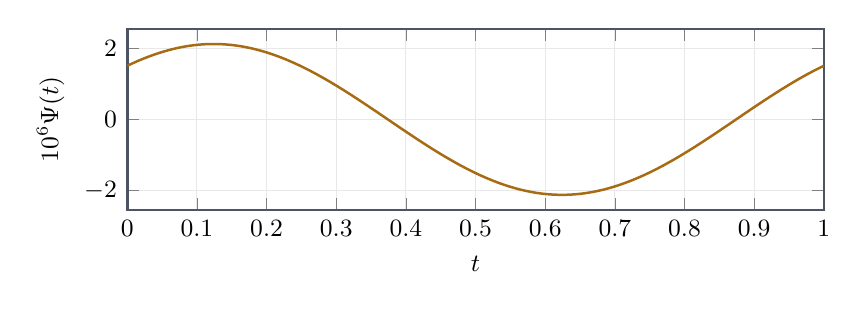
\begin{tikzpicture}
\begin{axis}[
 width=0.86\textwidth,height=0.32\textwidth,
 xmin=0,xmax=1,
 xlabel={$t$},ylabel={$10^6\PsiPer(t)$},
 grid=major,major grid style={draw=gray!18},
 axis line style={draw=FabiusGray},
 tick label style={font=\small},label style={font=\small},
 line width=0.9pt]
\addplot[draw=FabiusGold,smooth] coordinates {
(0,1.51172589466) (0.005,1.55790805556) (0.01,1.6025527476) (0.015,1.64561591208)
(0.02,1.6870550511) (0.025,1.72682926945) (0.03,1.76489931505) (0.035,1.80122761758)
(0.04,1.83577832566) (0.045,1.86851734215) (0.05,1.89941235785) (0.055,1.92843288334)
(0.06,1.95555027913) (0.065,1.98073778386) (0.07,2.00397054075) (0.075,2.02522562209)
(0.08,2.04448205193) (0.085,2.06172082671) (0.09,2.07692493406) (0.095,2.09007936956)
(0.1,2.10117115158) (0.105,2.11018933405) (0.11,2.11712501729) (0.115,2.12197135678)
(0.12,2.12472356993) (0.125,2.12537894077) (0.13,2.12393682266) (0.135,2.12039863891)
(0.14,2.11476788138) (0.145,2.10705010703) (0.15,2.09725293245) (0.155,2.08538602632)
(0.16,2.07146109988) (0.165,2.05549189537) (0.17,2.03749417249) (0.175,2.01748569281)
(0.18,1.99548620225) (0.185,1.97151741163) (0.19,1.94560297518) (0.195,1.91776846727)
(0.2,1.8880413571) (0.205,1.85645098165) (0.21,1.8230285167) (0.215,1.78780694604)
(0.22,1.750821029) (0.225,1.71210726603) (0.23,1.6717038628) (0.235,1.62965069241)
(0.24,1.58598925608) (0.245,1.54076264217) (0.25,1.49401548368) (0.255,1.44579391421)
(0.26,1.3961455224) (0.265,1.34511930499) (0.27,1.29276561847) (0.275,1.23913612936)
(0.28,1.18428376325) (0.285,1.12826265256) (0.29,1.07112808311) (0.295,1.01293643958)
(0.3,0.953745149844) (0.305,0.893612628312) (0.31,0.832598218276) (0.315,0.77076213335)
(0.32,0.708165398045) (0.325,0.644869787547) (0.33,0.580937766752) (0.335,0.516432428624)
(0.34,0.45141743193) (0.345,0.385956938415) (0.35,0.320115549486) (0.355,0.253958242458)
(0.36,0.187550306429) (0.365,0.120957277848) (0.37,0.0542448758411) (0.375,-0.012521062645)
(0.38,-0.0792746478179) (0.385,-0.145950002062) (0.39,-0.212481324952) (0.395,-0.278802958191)
(0.4,-0.344849450403) (0.405,-0.410555621731) (0.41,-0.475856628155) (0.415,-0.54068802549)
(0.42,-0.604985832985) (0.425,-0.668686596458) (0.43,-0.731727450924) (0.435,-0.794046182633)
(0.44,-0.855581290467) (0.445,-0.916272046636) (0.45,-0.976058556607) (0.455,-1.03488181822)
(0.46,-1.09268377989) (0.465,-1.14940739795) (0.47,-1.20499669289) (0.475,-1.25939680464)
(0.48,-1.3125540467) (0.485,-1.36441595909) (0.49,-1.41493136021) (0.495,-1.46405039723)
(0.5,-1.51172459541) (0.505,-1.55790690585) (0.51,-1.60255175196) (0.515,-1.64561507445)
(0.52,-1.68705437477) (0.525,-1.72682875711) (0.53,-1.76489896871) (0.535,-1.80122743861)
(0.54,-1.83577831476) (0.545,-1.86851749937) (0.55,-1.89941268256) (0.555,-1.92843337427)
(0.56,-1.95555093434) (0.565,-1.98073860076) (0.57,-2.00397151612) (0.575,-2.02522675208)
(0.58,-2.04448333208) (0.585,-2.06172225197) (0.59,-2.0769264988) (0.595,-2.09008106761)
(0.6,-2.10117297623) (0.605,-2.1101912781) (0.61,-2.11712707307) (0.615,-2.12197351618)
(0.62,-2.12472582443) (0.625,-2.12538128147) (0.63,-2.12393924032) (0.635,-2.12040112399)
(0.64,-2.11477042408) (0.645,-2.10705269731) (0.65,-2.09725556008) (0.655,-2.08538868093)
(0.66,-2.071463771) (0.665,-2.05549457246) (0.67,-2.03749684498) (0.675,-2.01748835015)
(0.68,-1.99548883397) (0.685,-1.97152000732) (0.69,-1.94560552461) (0.695,-1.91777096037)
(0.7,-1.88804378404) (0.705,-1.85645333285) (0.71,-1.82303078288) (0.715,-1.78780911826)
(0.72,-1.75082309868) (0.725,-1.71210922501) (0.73,-1.67170570334) (0.735,-1.62965240725)
(0.74,-1.58599083845) (0.745,-1.54076408582) (0.75,-1.49401678293) (0.755,-1.44579506392)
(0.76,-1.39614651804) (0.765,-1.34512014263) (0.77,-1.29276629479) (0.775,-1.2391366417)
(0.78,-1.18428410959) (0.785,-1.12826283153) (0.79,-1.07112809401) (0.795,-1.01293628236)
(0.8,-0.953744825129) (0.805,-0.893612137382) (0.81,-0.832597563068) (0.815,-0.77076131645)
(0.82,-0.708164422677) (0.825,-0.64486865756) (0.83,-0.580936486606) (0.835,-0.516431003371)
(0.84,-0.451415867194) (0.845,-0.385955240373) (0.85,-0.320113724838) (0.855,-0.253956298406)
(0.86,-0.187548250644) (0.865,-0.120955118444) (0.87,-0.0542426213404) (0.875,0.0125234033451)
(0.88,0.0792770654796) (0.885,0.145952487144) (0.89,0.212483867647) (0.895,0.278805548464)
(0.9,0.344852078031) (0.905,0.410558276344) (0.91,0.475859299277) (0.915,0.540690702579)
(0.92,0.604988505475) (0.925,0.668689253803) (0.93,0.731730082636) (0.935,0.794048778326)
(0.94,0.855583839898) (0.945,0.916274539743) (0.95,0.97606098355) (0.955,1.03488416942)
(0.96,1.09268604607) (0.965,1.14940957017) (0.97,1.20499876257) (0.975,1.25939876362)
(0.98,1.31255588723) (0.985,1.36441767393) (0.99,1.41493294258) (0.995,1.46405184089)
(1,1.51172589466)
};
\end{axis}
\end{tikzpicture}
\caption{The centered periodic correction, magnified by $10^6$.  The first Fourier
harmonic already gives visual accuracy.}
\label{fig:Psi-plot}
\end{figure}

\subsection{The lower Lambert phase}

The right coordinate is the large solution of
\begin{equation}\label{eq:lambda-saddle-equation}
  \Lam 2^{-\Lam}=x.
\end{equation}
For $0<\Ltwo x<e^{-1}$, define
\begin{equation}\label{eq:lambda-W-def}
  \Lam(x)=-\frac{W_{-1}(-\Ltwo x)}{\Ltwo},
  \qquad
  r(x)=2^{\Lam(x)}.
\end{equation}
Here $W_{-1}$ is the lower real branch of Lambert's $W$ function.

\begin{proposition}[Exact saddle coordinates]\label{prop:Lambert-coordinates}
For sufficiently small $x>0$,
\begin{equation}\label{eq:Lambert-identities}
  \Lam(x)2^{-\Lam(x)}=x,
  \qquad r(x)x=\Lam(x),
  \qquad \log r(x)=\Ltwo\Lam(x).
\end{equation}
Moreover $\Lam(x)\to\infty$ as $x\downarrow0$ and
\begin{equation}\label{eq:lambda-leading}
  \Lam(x)\sim\frac{-\log x}{\Ltwo}.
\end{equation}
\end{proposition}

\begin{proof}
The defining identity $W(z)e^{W(z)}=z$ with
$W=W_{-1}(-\Ltwo x)$ gives
$(-\Ltwo\Lam)e^{-\Ltwo\Lam}=-\Ltwo x$, proving the first formula.  The other two
are immediate.  The lower branch tends to $-\infty$ as its argument approaches
$0$ from below, so $\Lam\to\infty$.  Taking logarithms in
\eqref{eq:lambda-saddle-equation} gives
\begin{equation}\label{eq:lambda-log-equation}
  \Ltwo\Lam-\log\Lam=-\log x,
\end{equation}
from which \eqref{eq:lambda-leading} follows.
\end{proof}

For explicit conversion to elementary logarithms, put
\begin{equation}\label{eq:AB-phase}
  A=-\log(\Ltwo x),\qquad B=\log A.
\end{equation}
The solution $y=\Ltwo\Lam$ of $y-\log y=A$ has the standard expansion
\begin{equation}\label{eq:Lambert-phase-expansion}
\begin{split}
 \Ltwo\Lam={}&A+B+\frac BA
 +\frac{B-\tfrac12B^2}{A^2}\\
 &+\frac{B-\tfrac32B^2+\tfrac13B^3}{A^3}
 +O\left(\frac{B^4}{A^4}\right).
\end{split}
\end{equation}
The formal development proves the corresponding expansion to arbitrary order,
with explicit recursively generated polynomials in $B$.

For a dyadic argument $x=2^{-t}$, the phase $\Lam_t=\Lam(2^{-t})$ satisfies the
exact fixed-point relation
\begin{equation}\label{eq:dyadic-phase-fixed}
  \Lam_t-\frac{\log\Lam_t}{\Ltwo}=t,
\end{equation}
and therefore
\begin{equation}\label{eq:dyadic-phase-leading}
  \Lam_t=t+\frac{\log t}{\Ltwo}+o(1).
\end{equation}
The fractional part relevant to the periodic correction is
$\{\Lam_t\}$, not $\{t\}$.

\subsection{Exact Bromwich reduction}

The Laplace transform of the clamped CDF has a simple form.

\begin{lemma}[Laplace transform of $F$]\label{lem:F-Laplace}
For $\Re s>0$,
\begin{equation}\label{eq:F-Laplace}
  \int_0^{\infty}e^{-sx}F(x)\dd x=\frac{G(-s)}s.
\end{equation}
\end{lemma}

\begin{proof}
Stieltjes integration by parts on $[0,1]$ gives
\[
 G(-s)=\int_0^1e^{-sx}\dd F(x)
 =e^{-s}+s\int_0^1e^{-sx}F(x)\dd x.
\]
Since $F(x)=1$ for $x\ge1$,
$\int_1^\infty e^{-sx}\dd x=e^{-s}/s$.  Adding this tail proves
\eqref{eq:F-Laplace}.
\end{proof}

Fourier inversion of an exponentially tilted $F$ gives a Bromwich formula without
any contour-shifting hypothesis.  For every $r>0$,
\begin{equation}\label{eq:F-Bromwich}
 F(x)=e^{rx}\int_{\R}e^{2\pi\ii\xi x}
 \frac{G(-r-2\pi\ii\xi)}{r+2\pi\ii\xi}\dd\xi.
\end{equation}
Set $r=2^{\Lam}$ and use $rx=\Lam$.  After the change of variable
$\xi=rv/(2\pi\sqrt\Lam)$, define the normalized saddle mass
\begin{equation}\label{eq:saddle-mass-def}
 \mathcal S(x)=
 \frac{F(x)\sqrt{2\pi\Lam(x)}}
 {\exp(r(x)x+q(r(x)))}.
\end{equation}
Then exactly
\begin{equation}\label{eq:saddle-mass-integral}
 \mathcal S(x)=\frac1{\sqrt{2\pi}}\int_{\R}K_{\Lam(x)}(v)\dd v,
\end{equation}
where, using the analytic logarithm of $G(-z)$ in $\Re z>0$,
\begin{equation}\label{eq:saddle-kernel}
 K_\Lam(v)=\frac{1}{1+\ii v/\sqrt\Lam}
 \exp\left(
   \ii\sqrt\Lam\,v
   +q_{\C}\bigl(r(1+\ii v/\sqrt\Lam)\bigr)-q(r)
 \right).
\end{equation}
The real quantity $\mathcal S(x)$ is positive because $F(x)>0$.

Taking logarithms gives the exact identity
\begin{equation}\label{eq:exact-log-saddle}
 \log F(x)=r x+q(r)-\frac12\log(2\pi\Lam)+\log\mathcal S(x).
\end{equation}
No asymptotic approximation has yet been made.

\subsection{The corrected sharp main term}

Define
\begin{equation}\label{eq:Csharp-def}
 C=\frac{C_{\Gamma\zeta}}{\Ltwo}
   -\frac{7\Ltwo}{12}-\frac12\log\pi
 \approx-2.027983898638859424,
\end{equation}
and
\begin{equation}\label{eq:sharp-main}
 \mathcal M(x)=
 -\frac{\Ltwo}{2}\Lam(x)^2
 +\left(1+\frac{\Ltwo}{2}\right)\Lam(x)
 -\frac12\log\Lam(x)
 +C+\PsiPer(\Lam(x)).
\end{equation}

\begin{proposition}[Exact separation of the main term]\label{prop:exact-main-separation}
For small positive $x$, with $r=2^{\Lam(x)}$,
\begin{equation}\label{eq:exact-main-separation}
  r x+q(r)-\frac12\log(2\pi\Lam)
  =\mathcal M(x)+E(r).
\end{equation}
Consequently
\begin{equation}\label{eq:exact-error-separation}
  \log F(x)-\mathcal M(x)=\log\mathcal S(x)+E(r).
\end{equation}
\end{proposition}

\begin{proof}
Use $rx=\Lam$, $\log r=\Ltwo\Lam$, and the exact decomposition
\eqref{eq:q-periodic-decomposition}:
\[
 q(r)=-\frac{\Ltwo}{2}\Lam^2+\frac{\Ltwo}{2}\Lam
 +\overline R+\PsiPer(\Lam)+E(r).
\]
Now
\[
 \overline R-\frac12\log(2\pi)
 =\frac{C_{\Gamma\zeta}}{\Ltwo}-\frac{\Ltwo}{12}
  -\frac12\log2-\frac12\log\pi=C,
\]
because $(1/2)\log2=\Ltwo/2$.  Collecting terms proves
\eqref{eq:exact-main-separation}; combine it with
\eqref{eq:exact-log-saddle} to obtain \eqref{eq:exact-error-separation}.
\end{proof}

The analytic heart of the saddle argument is the following quantitative estimate.

\begin{theorem}[Normalized saddle mass]\label{thm:saddle-mass-leading}
As $x\downarrow0$,
\begin{equation}\label{eq:saddle-mass-leading}
  \mathcal S(x)=1+O\bigl(\Lam(x)^{-1}\bigr).
\end{equation}
\end{theorem}

\begin{proof}[Proof structure]
Put $\Lam=\Lam(x)$.  On a central arc
$|v|\le\Lam^{\delta}$ with a fixed small $\delta>0$, expand the analytic logarithm
in \eqref{eq:saddle-kernel}.  The identities $rx=\Lam$ and the explicit derivatives
of the periodic Laplace decomposition cancel the linear term and normalize the
quadratic term, giving
\begin{equation}\label{eq:kernel-leading-expansion}
  \log K_\Lam(v)=-\frac{v^2}{2}
  +O\left(\frac{1+|v|^3}{\sqrt\Lam}\right).
\end{equation}
A one-order-finer expansion shows that the term of order $\Lam^{-1/2}$ is odd and
purely imaginary, so its Gaussian integral vanishes.  The remaining central error
is $O(\Lam^{-1})$ after integration.

For the complementary arc, the infinite product
\eqref{eq:negative-Laplace-product} gives uniform vertical decay.  Factors whose
scale is comparable to $r$ provide a strict modulus loss away from the real axis;
additional factors give arbitrary polynomial decay.  This produces an integrable
majorant and makes the tail $o(\Lam^{-N})$ for the order needed here.  Thus
\eqref{eq:saddle-mass-integral} equals the normalized Gaussian integral
$(2\pi)^{-1/2}\int e^{-v^2/2}\dd v=1$ plus $O(\Lam^{-1})$.
\end{proof}

\begin{theorem}[Sharp endpoint asymptotic]\label{thm:sharp-asymptotic}
As $x\downarrow0$,
\begin{equation}\label{eq:sharp-log-asymptotic}
  \log F(x)=\mathcal M(x)+O\bigl(\Lam(x)^{-1}\bigr).
\end{equation}
Equivalently,
\begin{equation}\label{eq:sharp-multiplicative}
 F(x)=\frac{1}{\sqrt{\Lam(x)}}
 \exp\left(
 -\frac{\Ltwo}{2}\Lam(x)^2
 +\left(1+\frac{\Ltwo}{2}\right)\Lam(x)
 +C+\PsiPer(\Lam(x))
 \right)
 \left(1+O(\Lam(x)^{-1})\right).
\end{equation}
Since $\Lam(x)\asymp-\log x$, the logarithmic error is also
$O(1/(-\log x))$.
\end{theorem}

\begin{proof}
By \eqref{eq:exact-error-separation}, the error is
$\log\mathcal S(x)+E(r)$.  The estimate
\eqref{eq:saddle-mass-leading} and $\log(1+u)=u+O(u^2)$ give
$\log\mathcal S=O(\Lam^{-1})$.  The forward tail is
$E(2^\Lam)=O(e^{-2^\Lam})$, hence smaller than every inverse power of $\Lam$.
This proves \eqref{eq:sharp-log-asymptotic}; exponentiation gives
\eqref{eq:sharp-multiplicative}.
\end{proof}

\subsection{Compact Lambert-\texorpdfstring{$W$}{W} form}

Let
\begin{equation}\label{eq:W-short}
  W=W_{-1}(-\Ltwo x),\qquad \Lam=-W/\Ltwo.
\end{equation}
The sharp main term \eqref{eq:sharp-main} is identically equal to
\begin{equation}\label{eq:compact-W-main}
 \mathcal M_W(x)=
 -\frac{7\Ltwo}{12}-\frac12\log(\pi x)
 +\frac{C_{\Gamma\zeta}-W-\tfrac12W^2}{\Ltwo}
 +\PsiPer\left(-\frac W{\Ltwo}\right).
\end{equation}
Indeed, $\log x=\log\Lam-\Ltwo\Lam$ and $W=-\Ltwo\Lam$ reduce
\eqref{eq:compact-W-main} to \eqref{eq:sharp-main}.  Therefore
\begin{equation}\label{eq:compact-W-asymptotic}
  \log F(x)=\mathcal M_W(x)+O\left(\frac1{-\log x}\right).
\end{equation}
This is the shortest correct version of the leading asymptotic.

\subsection{Expansion in elementary logarithms}

Some applications prefer not to leave Lambert $W$ in the answer.  Put
\begin{equation}\label{eq:T-H-a}
  T=-\log x,\qquad H=\log T,\qquad a=\log\Ltwo.
\end{equation}
Define
\begin{equation}\label{eq:C0-elementary}
 C_0=
 \frac{6\gamma^2+12\gamma_1-\pi^2-6a^2}{12\Ltwo}
 -\frac{7\Ltwo}{12}-\frac12\log\pi.
\end{equation}
Then set
\begin{equation}\label{eq:elementary-main}
\begin{split}
 \mathcal M_{\mathrm{elem}}(x)={}&
 -\frac{T^2}{2\Ltwo}-\frac{TH}{\Ltwo}
 +\left(\frac12+\frac{1+a}{\Ltwo}\right)T\\
 &-\frac{H^2}{2\Ltwo}+\frac{aH}{\Ltwo}+C_0
 -\frac{H^2}{2\Ltwo T}+\frac{aH}{\Ltwo T}.
\end{split}
\end{equation}

\begin{theorem}[Elementary-logarithm form]\label{thm:elementary-asymptotic}
As $x\downarrow0$,
\begin{equation}\label{eq:elementary-asymptotic}
  \log F(x)=\mathcal M_{\mathrm{elem}}(x)
  +\PsiPer(\Lam(x))+O(T^{-1}).
\end{equation}
\end{theorem}

\begin{proof}
Insert the Lambert expansion \eqref{eq:Lambert-phase-expansion} into the
nonoscillatory part of \eqref{eq:sharp-main}, retain all terms that are not
$o(T^{-1})$, and simplify.  This gives exactly
\eqref{eq:elementary-main}.  The saddle error is already $O(T^{-1})$.
Crucially, the periodic term is \emph{not} expanded by replacing $\Lam$ with a
coarse approximation: an $o(1)$ phase error can still change a nonconstant
periodic function by an amount larger than the desired remainder.  It must remain
sampled at the exact lower-Lambert phase, or the phase itself must be expanded to
matching precision and then propagated through the derivatives of $\PsiPer$.
\end{proof}

For the dyadic scale $x=2^{-t}$, a convenient nonoscillatory main term is
\begin{equation}\label{eq:dyadic-elementary-main}
\begin{split}
 \mathcal M_{\mathrm{dyad}}(t)={}&
 -\frac{\Ltwo}{2}t^2-t\log t
 +\left(1+\frac{\Ltwo}{2}\right)t
 -\frac{(\log t)^2}{2\Ltwo}+C\\
 &-\frac{(\log t)^2}{2\Ltwo^2t}.
\end{split}
\end{equation}
Then
\begin{equation}\label{eq:dyadic-elementary-asymptotic}
  \log F(2^{-t})=\mathcal M_{\mathrm{dyad}}(t)
  +\PsiPer(\Lam_t)+O(t^{-1}).
\end{equation}
Substituting $T=\Ltwo t$ into \eqref{eq:elementary-main} differs from
\eqref{eq:dyadic-elementary-main} by only
$(\log\Ltwo)^2/(2\Ltwo^2t)$, already within the stated error.

\subsection{Why the periodic term cannot be omitted}

\begin{warningbox}[A common but genuine asymptotic error]
A formula of the form
\[
  \log F(x)=\mathcal M_{\mathrm{elem}}(x)
  +O\left(\frac1{-\log x}\right)
\]
with no periodic correction is false.  The missing term is tiny numerically, but it
is of order $1$, not of order $1/\log x$.
\end{warningbox}

\begin{proposition}[Obstruction to a nonoscillatory remainder]\label{prop:periodic-obstruction}
Let $M_0(x)$ be any main term satisfying
$M_0(x)=\mathcal M(x)-\PsiPer(\Lam(x))+o(1)$.  Then
\begin{equation}\label{eq:no-small-remainder}
  \log F(x)-M_0(x)\not\longrightarrow0
\end{equation}
unless $\PsiPer$ is identically zero.
\end{proposition}

\begin{proof}
For a fixed $u\in[0,1)$, choose
\begin{equation}\label{eq:phase-subsequence}
  \Lam_n=n+u,
  \qquad x_n=\Lam_n2^{-\Lam_n}.
\end{equation}
Then $x_n\downarrow0$ and the exact Lambert phase of $x_n$ is $\Lam_n$.  The sharp
theorem gives
\[
 \log F(x_n)-M_0(x_n)=\PsiPer(n+u)+o(1)=\PsiPer(u)+o(1).
\]
If the left side tended to zero for all such sequences, then $\PsiPer(u)=0$ for
every $u$.  This contradicts the nonzero Fourier coefficient
\eqref{eq:first-Psi-coeff-numeric}.
\end{proof}

\subsection{The first saddle correction}

The normalized saddle mass has a full asymptotic expansion.  Its first nontrivial
term can be written explicitly using the derivatives of $\PsiPer$.  Define
\begin{align}
 A(u)&=\frac{\PsiPer'(u)}{\Ltwo}-\frac12,
 \label{eq:A-first-correction}\\
 B(u)&=-\frac14+\frac1{2\Ltwo}
 +\frac{\PsiPer'(u)}{2\Ltwo}
 -\frac{\PsiPer''(u)}{2\Ltwo^2}.
 \label{eq:B-first-correction}
\end{align}
On the central scale, the exponent in the saddle kernel has the form
\begin{equation}\label{eq:first-kernel-expansion}
 \log K_\Lam(v)=
 -\frac{v^2}{2}
 +\Lam^{-1/2}P_1(v;u)
 +\Lam^{-1}P_2(v;u)
 +O\bigl(\Lam^{-3/2}(1+|v|^9)\bigr),
\end{equation}
where $u=\Lam$ modulo $1$ and
\begin{equation}\label{eq:P1-P2}
  P_1(v;u)=\ii\left(A(u)v+\frac{v^3}{3}\right),
  \qquad
  P_2(v;u)=\frac{v^4}{4}+B(u)v^2.
\end{equation}
The $\Lam^{-1/2}$ contribution integrates to zero by oddness.  At order
$\Lam^{-1}$, let $Z$ be standard normal.  The relative mass coefficient is
\begin{align}
 m_1(u)
 &=\E\left[P_2(Z;u)+\frac12P_1(Z;u)^2\right]\notag\\
 &=\frac34+B(u)-\frac12\left(A(u)^2+2A(u)+\frac53\right).
 \label{eq:m1-Gaussian}
\end{align}
Using $\E Z^2=1$, $\E Z^4=3$, and $\E Z^6=15$, simplification gives
\begin{equation}\label{eq:alpha1}
 \alpha_1(u)=
 \frac1{24}+\frac1{2\Ltwo}
 -\frac{\PsiPer''(u)+(\PsiPer'(u))^2}{2\Ltwo^2}.
\end{equation}

\begin{theorem}[First corrected saddle term]\label{thm:first-saddle-correction}
As $x\downarrow0$,
\begin{equation}\label{eq:first-saddle-correction}
 \log F(x)=\mathcal M(x)
 +\frac{\alpha_1(\Lam(x))}{\Lam(x)}
 +O\bigl(\Lam(x)^{-2}\bigr).
\end{equation}
The coefficient $\alpha_1$ is smooth and one-periodic.
\end{theorem}

\begin{proof}
Exponentiate \eqref{eq:first-kernel-expansion}, integrate termwise against the
normalized Gaussian, and use \eqref{eq:m1-Gaussian}.  This gives
$\mathcal S(x)=1+\alpha_1(\Lam)/\Lam+O(\Lam^{-2})$.  Taking the logarithm does not
change the first coefficient.  The forward tail remains exponentially small, so
\eqref{eq:exact-error-separation} proves the result.
\end{proof}

\subsection{The all-orders expansion}

\begin{theorem}[Full Poincare expansion]\label{thm:full-asymptotic}
There exist smooth one-periodic functions $\alpha_j\colon\R\to\R$ for $j\ge1$
such that, for every integer $N\ge1$,
\begin{equation}\label{eq:full-asymptotic}
 \log F(x)=\mathcal M(x)
 +\sum_{j=1}^{N-1}\frac{\alpha_j(\Lam(x))}{\Lam(x)^j}
 +O\bigl(\Lam(x)^{-N}\bigr)
 \qquad(x\downarrow0).
\end{equation}
The first coefficient is \eqref{eq:alpha1}.  Every $\alpha_j$ is obtained by a
finite algebraic-differential expression in $\PsiPer$ and its derivatives, with
coefficients in $\Q(\Ltwo)$.
\end{theorem}

\begin{proof}[Construction and proof]
Expand the logarithm of the scaled kernel to arbitrary order:
\begin{equation}\label{eq:all-order-kernel-log}
 \log K_\Lam(v)=-\frac{v^2}{2}
 +\sum_{m=1}^{2N}\Lam^{-m/2}P_m(v;\Lam)
 +\mathcal R_N(v,\Lam).
\end{equation}
Each $P_m$ is a polynomial in $v$ whose coefficients are smooth periodic
combinations of derivatives of $\PsiPer$.  Uniform derivative bounds follow from
the absolutely convergent Fourier series \eqref{eq:Psi-Fourier-series}.  Taylor's
theorem gives a central-arc bound on $\mathcal R_N$; the vertical product estimates
make the complementary arc smaller than $\Lam^{-N}$.

Exponentiating \eqref{eq:all-order-kernel-log} produces complete Bell polynomials
in $P_1,P_2,\ldots$.  Integrating termwise against $e^{-v^2/2}$ replaces every
monomial by a Gaussian moment.  Odd half-integer powers vanish by parity, leaving
\begin{equation}\label{eq:mass-full-expansion}
  \mathcal S(x)=1+\sum_{j=1}^{N-1}
  \frac{m_j(\Lam(x))}{\Lam(x)^j}+O(\Lam^{-N}),
\end{equation}
with smooth periodic $m_j$.

Finally, write
$1+\sum_{j\ge1}m_jz^j=\exp(\sum_{j\ge1}\alpha_jz^j)$.  Comparing derivatives
gives the finite recursion
\begin{equation}\label{eq:log-coefficient-recursion}
  \alpha_n=m_n-\frac1n\sum_{k=1}^{n-1}
  k\alpha_km_{n-k},\qquad n\ge1.
\end{equation}
This defines the periodic logarithmic coefficients.  Insert the resulting expansion
of $\log\mathcal S$ into \eqref{eq:exact-error-separation}; the forward tail
$E(2^\Lam)$ is beyond all algebraic orders and does not affect any coefficient.
\end{proof}

\begin{remark}[Two independent all-orders operations]
There are two distinct expansions:
\begin{enumerate}
\item the saddle expansion in powers of $1/\Lam$, whose coefficients are periodic;
\item the Lambert-phase expansion of $\Lam$ in powers of $1/(-\log x)$ with
      polynomial logarithmic coefficients.
\end{enumerate}
They can be composed, but the periodic phase must be propagated to the same order.
Blindly replacing $\Lam$ by the first two elementary terms inside $\PsiPer(\Lam)$
loses control of the claimed remainder.
\end{remark}

\section{Synthesis and computational workflow}\label{sec:synthesis}

The theory is unusually coherent: each viewpoint supplies the difficult step for a
different class of questions.

\begin{center}
\begin{tabularx}{0.95\textwidth}{>{\bfseries}p{0.20\textwidth}X}
\toprule
Viewpoint & What it makes transparent\\
\midrule
Probability & Existence, positivity, symmetry, support, weak convergence, the
negative Laplace product.\\
Infinite convolution & Smoothness, constructive approximation, Fourier product,
rapid decay.\\
Delay equation & Self-similarity, endpoint flatness, derivative identities.\\
Thue--Morse extension & A global dilation equation, exact dyadic derivatives,
closed rational formulas.\\
Moments & Rational recurrences, inverse-power values, denominator control.\\
Taylor blocks & Fast exact evaluation following the $1$-bits of the numerator.\\
Poisson summation & Partition of unity, sampling identities, cosine expansion.\\
Legendre analysis & Exact orthogonal coefficients and optimal polynomial
approximation.\\
Negative Laplace analysis & Log-periodic structure and the Gamma--zeta correction.\\
Lambert saddle analysis & The sharp endpoint expansion and all higher corrections.\\
\bottomrule
\end{tabularx}
\end{center}

For exact arithmetic at a dyadic $a/2^N$, the recommended workflow is:
\begin{enumerate}
\item generate $d_0,\ldots,d_N$ by \eqref{eq:d-recurrence};
\item use \cref{alg:dyadic-evaluator} to remove highest binary digits;
\item use the closed formula \eqref{eq:closed-dyadic} independently when a
      denominator certificate or a cross-check is desired;
\item derive exact derivatives from \eqref{eq:exact-dyadic-derivative};
\item reduce the resulting rational only at controlled points if expression swell
      matters.
\end{enumerate}
For tiny non-dyadic $x$, the sharp asymptotic should be evaluated in this order:
\begin{enumerate}
\item compute the lower-branch phase $\Lam=-W_{-1}(-x\log2)/\log2$;
\item compute the rapidly convergent Fourier series for $\PsiPer(\Lam)$, normally
      using only its first harmonic at ordinary precision;
\item evaluate \eqref{eq:sharp-main} or \eqref{eq:compact-W-main};
\item add $\alpha_1(\Lam)/\Lam$ if a second-order logarithmic approximation is
      needed.
\end{enumerate}
The exact phase is cheap compared with the enormous dynamic range of $F(x)$, and
retaining it avoids the only structurally serious error in the naive elementary
formula.

\section{Corrections and strengthened statements}\label{sec:corrections}

A formal development is particularly useful for this topic because many formulas
are correct in spirit but sensitive to endpoint conventions, global-versus-bounded
notation, or a single power of two.  The development underlying this article makes
the following points explicit.

\begin{enumerate}
\item \textbf{Bounded versus signed Fabius functions.}
The clamped $F\colon\R\to[0,1]$ does not satisfy $F'(x)=2F(2x)$ for all positive
$x$; the signed extension $\Thetaf$ does.  Every global derivative formula in this
article is stated for $\Thetaf$, then restricted to $[0,1]$ when appropriate.

\item \textbf{Finite convolution approximants.}
At a finite stage one must convolve only the finite family of uniform kernels that
has actually been introduced.  An infinite-convolution notation at a finite step
obscures the induction and is not literally correct.

\item \textbf{Endpoint weights in step approximants.}
The indicator of a closed dyadic cell must carry half-weight at its endpoints if
the stated pointwise convergence is intended to include grid boundaries.  The
interior convergence is unaffected, but the literal endpoint theorem otherwise
fails.

\item \textbf{Poisson summation.}
The translated formula is
\[
 \sum_m\upf(t+am)=a^{-1}\sum_k\Fourier(k/a)e^{2\pi\ii kt/a};
\]
the translation parameter and exponential factor cannot be omitted.  Statements
with a positive integer subdivision parameter require that parameter to be
strictly positive.

\item \textbf{Removable singularities.}
The factor $(e^z-1)/z$ in \eqref{eq:f-functional} is an entire function after
assigning the value $1$ at $z=0$.  Coefficient arguments should use this completed
function rather than silently divide by zero.

\item \textbf{Taylor-remainder hypotheses.}
The translated-remainder lemma behind \cref{thm:Taylor-reduction} needs the scale
and derivative order to stay in the range where the iterated dilation formula is
valid.  The formal theorem records the missing inequality instead of relying on an
implicit convention about negative indices.

\item \textbf{The sign of the Reshetnikov exponent.}
The definition is
$2^{\binom{n-1}{2}}(2n)!F(2^{-n})\cdots$, with a positive exponent as in
\eqref{eq:R-number-def}.  A negative exponent would contradict the integral values
already at small indices.

\item \textbf{Normalization of the closed dyadic formula.}
The powers of two in the Taylor-integral change of variables must be tracked
through both the polynomial factor and the differential.  The normalized form is
\eqref{eq:closed-dyadic}; it is stable under dyadic refinement and agrees with the
exact evaluator.

\item \textbf{The sharp asymptotic needs a periodic term.}
The nonconstant function $\PsiPer(\Lam(x))$ in
\eqref{eq:sharp-log-asymptotic} cannot be absorbed into an
$O(1/(-\log x))$ remainder.  The subsequence argument in
\cref{prop:periodic-obstruction} gives a direct disproof of the uncorrected claim.

\item \textbf{All-orders expansion requires exact phase bookkeeping.}
The saddle coefficients are periodic functions of the lower-Lambert phase.  A
truncated expansion of $\Lam$ may be substituted only after its error has been
propagated through the derivatives of those periodic coefficients.
\end{enumerate}

\appendix

\section{Correspondence with the Lean development}\label{app:Lean-map}

The proof organization above follows the dependency graph of the Lean source rather
than the order of the historical papers.  The table lists representative modules;
several technical bridge files are omitted from the right column for readability.

\footnotesize
\begin{longtable}{>{\raggedright\arraybackslash}p{0.25\textwidth}>{\raggedright\arraybackslash}p{0.67\textwidth}}
\toprule
Mathematical topic & Representative Lean modules\\
\midrule
\endfirsthead
\toprule
Mathematical topic & Representative Lean modules\\
\midrule
\endhead
Bounded specification, regularity, and the $F$--$\upf$ bridge &
\texttt{Basic.lean}, \texttt{OriginalPaperSupplement.lean}\\
Probability, moments, and generating functions &
\texttt{AnalyticMoments.lean}, \texttt{Paper05442.lean}\\
Closed dyadic values and the exact evaluator &
\texttt{DyadicClosedForm.lean}, \texttt{TaylorReduction.lean}\\
Arithmetic sequences and denominator results &
\texttt{Arithmetic.lean}, \texttt{PaperStatements.lean}\\
Finite $q$-binomial and Thue--Morse identities &
\texttt{FabiusQBinomialFormula.lean};\newline
\texttt{FabiusDyadicQBinomialScalar.lean}\\
Legendre coefficients and approximation &
\texttt{FabiusLegendreCoefficients.lean}\\
Negative Laplace product and periodic correction &
\texttt{NegativeLaplace.lean}; \texttt{PeriodicCorrection.lean};\newline
\texttt{PeriodicMean.lean}\\
Lower Lambert phase and explicit saddle radius &
\texttt{FabiusLambertPhase.lean}, \texttt{FabiusLambertSaddle.lean}\\
Bromwich inversion and exact saddle reduction &
\texttt{FabiusBromwichInput.lean}; \texttt{FabiusSaddleReduction.lean};\newline
\texttt{FabiusSharpExactReduction.lean}\\
Sharp main term and elementary logarithmic form &
\texttt{FabiusSharpConstant.lean}; \texttt{FabiusSharpLambertMain.lean};\newline
\texttt{FabiusWikipediaMain.lean}; \texttt{FabiusWikipediaExpansion.lean}\\
First and all-orders saddle corrections &
\texttt{FabiusFirstSaddleCorrection.lean};\newline
\texttt{FabiusFullAsymptoticExpansion.lean}\\
Coverage and audit &
Repository-level \texttt{README.md}; \texttt{PAPER\_COVERAGE.md};\newline
\texttt{ASYMPTOTIC\_COMPLETION\_AUDIT.md}\\
\bottomrule
\end{longtable}
\normalsize

The formal source separates statements over $\R$, $\C$, and $\Q$ more sharply than
an ordinary exposition does.  In particular, the exact evaluator lives over the
rationals and is later cast to the reals; the analytic uniqueness theorem then
shows that its real value is independent of the chosen representative satisfying
the Fabius axioms.  This separation is what turns ``the algorithm appears to work''
into a theorem about the unique mathematical function.

\section{Selected exact data}\label{app:data}

For convenient checking, here are several sequences in aligned form.

\subsection*{Moments}
\begin{align*}
(c_n)_{n\ge0}={}&1,\ \frac19,\ \frac{19}{675},\ \frac{583}{59535},
 \frac{132809}{32531625},\ \frac{46840699}{24405225075},\ldots,\\
(d_n)_{n\ge0}={}&1,\ \frac12,\ \frac5{18},\ \frac16,\ \frac{143}{1350},
 \frac{19}{270},\ \frac{1153}{23814},\ \frac{583}{17010},\ldots.
\end{align*}

\subsection*{Inverse-power values}
\begin{align*}
F(1)&=1,& F(1/2)&=\frac12,& F(1/4)&=\frac5{72},\\
F(1/8)&=\frac1{288},&
F(1/16)&=\frac{143}{2\,073\,600},&
F(1/32)&=\frac{19}{33\,177\,600},\\
F(1/64)&=\frac{1153}{561\,842\,749\,440},&
F(1/128)&=\frac{583}{179\,789\,679\,820\,800}.&&
\end{align*}

\subsection*{Asymptotic constants}
\begin{align*}
 \Ltwo&=0.6931471805599453094\ldots,\\
 C_{\Gamma\zeta}&=-0.7286939170039306059\ldots,\\
 \overline R&=-1.1090453654341866822\ldots,\\
 C&=-2.0279838986388594240\ldots.
\end{align*}
The magnitude of the first periodic Fourier coefficient is
$1.0627109779221651\times10^{-6}$; the second is already about
$6.69\times10^{-13}$.

\section{Notation index}\label{app:notation}

\begin{longtable}{p{0.18\textwidth}p{0.72\textwidth}}
\toprule
Symbol & Meaning\\
\midrule
$F$ & Bounded, clamped Fabius CDF, equal to $0$ on $(-\infty,0]$ and $1$ on
$[1,\infty)$.\\
$\upf$ & Rvachev's even $C^\infty$ bump supported on $[-1,1]$.\\
$\Thetaf$ & Signed Thue--Morse global extension of $F$.\\
$\wt(n)$ & Number of $1$-bits in $n$.\\
$\epsTM_n$ & Thue--Morse sign $(-1)^{\wt(n)}$.\\
$c_n$ & Even moment $\int x^{2n}\upf(x)\dd x$.\\
$d_n$ & Half-moment $n\int_0^1x^{n-1}\upf(x)\dd x$, with $d_0=1$.\\
$\mathsf F_n,\mathsf G_n$ & Integral numerator sequences associated with $c_n,d_n$.\\
$R_n$ & Reshetnikov number in \eqref{eq:R-number-def}.\\
$D_n$ & Common denominator of reduced odd-grid values at level $n$.\\
$G(z)$ & Moment generating function $\E(e^{zX})$.\\
$q(s)$ & $\log G(-s)$ for $s>0$.\\
$R(t)$ & Exact one-periodic correction in the negative Laplace logarithm.\\
$\PsiPer(t)$ & Centered periodic correction $R(t)-\overline R$.\\
$\Lam(x)$ & Lower-Lambert phase solving $\Lam2^{-\Lam}=x$.\\
$\mathcal S(x)$ & Normalized saddle mass in \eqref{eq:saddle-mass-def}.\\
$\mathcal M(x)$ & Corrected sharp logarithmic main term in \eqref{eq:sharp-main}.\\
\bottomrule
\end{longtable}

\clearpage
\begin{thebibliography}{99}

\bibitem{Arias1982}
J.~Arias de Reyna,
\emph{Definici\'on y estudio de una funci\'on indefinidamente diferenciable de
soporte compacto},
Rev. Real Acad. Cienc. Exact. F\'is. Natur. Madrid \textbf{76} (1982), 21--38.
English translation: \emph{An infinitely differentiable function with compact
support: Definition and Properties}, arXiv:1702.05442.

\bibitem{AriasArithmetic}
J.~Arias de Reyna,
\emph{Arithmetic of the Fabius function},
arXiv:1702.06487, version 3, 2017.

\bibitem{Fabius1966}
J.~Fabius,
\emph{A probabilistic example of a nowhere analytic $C^\infty$-function},
Z. Wahrscheinlichkeitstheorie verw. Gebiete \textbf{5} (1966), 173--174.

\bibitem{Fine1947}
N.~J. Fine,
\emph{Binomial coefficients modulo a prime},
Amer. Math. Monthly \textbf{54} (1947), 589--592.

\bibitem{Haugland2016}
J.~K. Haugland,
\emph{Evaluating the Fabius function},
arXiv:1609.07999, 2016.

\bibitem{JessenWintner1935}
B.~Jessen and A.~Wintner,
\emph{Distribution functions and the Riemann zeta function},
Trans. Amer. Math. Soc. \textbf{38} (1935), 48--88.

\bibitem{Rvachev1971}
V.~L. Rvachev and V.~A. Rvach\"ev,
\emph{A certain finite function},
Dopov\={\i}d\={\i} Akad. Nauk Ukra\={\i}n. RSR Ser. A (1971), 705--707, 764.

\bibitem{Rvachev1973}
V.~A. Rvach\"ev,
\emph{Certain functions with compact support, and their applications},
1973, 139--149, 194 (Russian).

\bibitem{Rvachev1990}
V.~A. Rvach\"ev,
\emph{Compactly-supported solutions of functional-differential equations and
their applications},
Uspekhi Mat. Nauk \textbf{45} (1990), no.~1, 77--103, 222 (Russian).

\bibitem{CorlessW}
R.~M. Corless, G.~H. Gonnet, D.~E. G. Hare, D.~J. Jeffrey, and D.~E. Knuth,
\emph{On the Lambert $W$ function},
Adv. Comput. Math. \textbf{5} (1996), 329--359.

\bibitem{ProveIt}
V.~Reshetnikov,
\emph{ProveIt: Analysis/FabiusFunction},
Lean formalization and accompanying audits,
\url{https://github.com/VladimirReshetnikov/ProveIt/tree/main/Analysis/FabiusFunction},
accessed August 2026.

\end{thebibliography}

\end{document}
